%!TEX encoding = UTF-8 Unicode

%% Projeto em Engenharia Aeroespacial 2023/24
%% Template para relattórios preliminar e final 
%%
%% Based on the example.tex file provided by Tomás Oliveira e Silva
%%
%% Modified by João Paulo Barraca <jpbarraca@ua.pt>
%% Modified by Filipe Manco <filipe.manco@ua.pt>
%% Modified by Pedro Casau <pcasau@ua.pt>

% Add 'final' parameter to remove "Relatório Intermédio" from cover page
\documentclass[11pt,oneside,a4paper,final]{report}

\usepackage[engineering,deti]{uaThesisTemplate}

%% Optional packages for utf8 encoding and T1 fonts
\usepackage[utf8]{inputenc}
\usepackage[T1]{fontenc}

%% For prettier pages
\usepackage{lmodern}

%% We will use english and portuguese
\usepackage[english,portuguese]{babel}

\usepackage{xspace}% used by \sigla
\usepackage{amsmath}          % aligned equations, split, etc.
\usepackage{amssymb}          % mathematical symbols
\usepackage{amsthm}           % theorem environments
\usepackage{mathtools}        % extensions to amsmath
\usepackage{bm}               % bold math symbols (\bm{})
\usepackage{isomath}          % ISO 80000 math formatting
\usepackage{siunitx}


% ── FIGURES & GRAPHICS ───────────────────────────────────────────
\usepackage{graphicx}         % \includegraphics
\usepackage{float}            % [H] float placement
\usepackage{subfig}           % subfigures (a), (b), ...
\usepackage{wrapfig}          % text wrapping around figures
\usepackage{tikz}             % vector drawings (Collar triangle)
\usetikzlibrary{shapes, arrows.meta, positioning, calc}
\usepackage{pgfplots}         % plots inside LaTeX
\pgfplotsset{compat=1.18}
\usepackage[numbers,sort&compress]{natbib}
\usepackage{url}


% ── TABLES ───────────────────────────────────────────────────────
\usepackage{booktabs}         % professional table rules
\usepackage{multirow}         % merge rows in tables
\usepackage{multicol}         % merge columns
\usepackage{array}            % extended column types
\usepackage{tabularx}         % auto-width columns
\usepackage{longtable}        % tables spanning multiple pages
\usepackage{colortbl}         % coloured table cells
\usepackage{xcolor}     


%%%%%%%%%%%%%%%%%%%%%%%%%%%%%%%%%%%%%%%%%%%%%%%%%%
%%       DEFINE COVER FIELDS
%%                  START
%%%%%%%%%%%%%%%%%%%%%%%%%%%%%%%%%%%%%%%%%%%%%%%%%%


%%% Edit author's name
%% Author's full name
\Author{Alexandre Cauvel\\ Diego Mota}

%%% Edit title in Portuguese
\TitlePT{Análise Modal da Asa do Antonov AN-124: Influência da Orientação das Nervuras nas Frequências Naturais e Formas Modais}

%%% OPTIONAL: you can write your title in
%%%  other languages. You can repeat the following
%%%  line as many times as you want, or remove it
%%%  if you only want the portuguese title.
%% Optional Titles in additional languages.
%\TitleEN{TITLE (MAX 70 CHARACTERS)}

%%% OPTIONAL: edit grant support texts where
%%%  appropriate. Maximum two.
%%%
%%% \GrantText{grant1}{grant2}
%% Optional Grant support texts
%\GrantText{Texto Apoio financeiro do POCTI no âmbito do III Quadro Comunitário de Apoio.}
%          {Texto Apoio financeiro da FCT e do FSE no âmbito do III Quadro Comunitário de Apoio.}

%%% OPTIONAL: Add a dedication text.
%% Optional Dedication text
%\Dedication{Dedico este trabalho à minha esposa e filho pelo incansável apoio.}

%%% OPTIONAL: Add an acknowledgement text
%% Optional Acknowledgement text
%\Acknowledgements{Agradeço toda a ajuda a todos os meus colegas e companheiros.}

%%% Edit the keywords and abstract in Portuguese
%%  Keywords and Abstract in Portuguese
\Abstract{Palavras Chave}{aeroelasticidade, frequências naturais, formas modais, análise modal, elementos finitos, Antonov AN-124, orientação das nervuras, NX Nastran.}{Resumo}{\selectlanguage{portuguese}O presente trabalho insere-se no âmbito da unidade curricular de Aeroelasticidade da licenciatura em Engenharia Aeroespacial e tem como objetivo o estudo da influência da orientação das nervuras (\textit{ribs}) sobre as frequências naturais e formas modais de uma asa de aeronave. A aeronave de referência escolhida foi o Antonov AN-124 \textit{Ruslan}, tendo sido desenvolvido um modelo numérico simplificado e reduzido à escala de aproximadamente 1:9, com semi-envergadura de 4~m, no software SolidWorks, e posteriormente importado para o NX Siemens para a realização da análise modal.
A estrutura alar foi discretizada com elementos de casca quadrilaterais de segunda ordem CQUAD8, sendo o revestimento modelado em liga de alumínio 2024-T3 e as longarinas e nervuras em liga de alumínio 7075-T6. Foram estudadas duas configurações de orientação das nervuras: a Configuração A, com nervuras inclinadas a 25° relativamente ao plano de simetria da aeronave (aproximadamente perpendiculares ao bordo de ataque), e a Configuração B, com nervuras paralelas ao plano de simetria. A análise modal foi executada no NX Nastran através da solução SOL~103 com o método de Lanczos, extraindo os primeiros 10 modos de vibração para cada configuração.
Os resultados mostram que a alteração da orientação das nervuras introduz variações nas frequências naturais inferiores a 1\% nos primeiros quatro modos de interesse (1B, 2B, 3B e 1T), contrariamente à hipótese teórica inicial que previa um efeito mais pronunciado nos modos de torção. A rigidez torsional da caixa alar revelou ser dominada pela contribuição do revestimento e das longarinas, comuns a ambas as configurações, e não pela orientação das nervuras. Contudo, a análise da totalidade dos 10 modos extraídos revelou que a Configuração B apresenta uma maior densidade de modos de torção a frequências mais baixas, confirmando parcialmente a hipótese teórica e evidenciando a importância de considerar um número suficiente de modos na análise modal de estruturas alares.}


%%%%%%%%%%%%%%%%%%%%%%%%%%%%%%%%%%%%%%%%%%%%%%%%%%
%%       DEFINE COVER FIELDS
%%                  END
%%%%%%%%%%%%%%%%%%%%%%%%%%%%%%%%%%%%%%%%%%%%%%%%%%


\begin{document}

%%% By default we consider portuguese to be the
%%%  main language (the last one in the usepackage
%%%  declaration). If you're writing your document
%%%  in english uncomment the following line.
%%% Set the proper language or you will end with incorrect hyphenation!
\selectlanguage{portuguese}

\MakeCover

% Disable addition of ToC, LoF and LoT to the table of contents
\addtocontents{toc}{\protect\setcounter{tocdepth}{-1}}

\tableofcontents

\listoffigures
\listoftables

\newpage

% Restore the default value (chapter-level)
\addtocontents{toc}{\protect\setcounter{tocdepth}{2}}

\chapter{Introdução}
\label{chap:introducao}

\section{Contextualização e Motivação}

A aeroelasticidade é uma das disciplinas mais críticas no projeto de aeronaves modernas, estabelecendo a ponte entre a aerodinâmica, a dinâmica estrutural e a mecânica do voo. À medida que as aeronaves evoluem para estruturas mais leves e flexíveis, tendência impulsionada pela necessidade de reduzir o consumo de combustível e aumentar a eficiência operacional, os fenómenos aeroelásticos assumem um papel cada vez mais preponderante no projeto e na certificação \cite{Wright2015, Dowell2004}.

No contexto das aeronaves de transporte pesado, a asa é o componente estrutural mais sujeito a efeitos aeroelásticos relevantes. A sua grande envergadura, a flexibilidade inerente às estruturas de parede fina e a presença de cargas aerodinâmicas distribuídas de grande magnitude tornam a análise do seu comportamento dinâmico indispensável nas fases iniciais de projeto \cite{Megson2012, Bisplinghoff1996}. A determinação das frequências naturais e das formas modais da asa constitui, em particular, uma etapa preliminar indispensável para qualquer análise aeroelástica. Com esta base estrutural, é possível avaliar tanto fenómenos estáticos, como a divergência e a inversão de controlos, quanto comportamentos dinâmicos, nomeadamente o \textit{flutter} e a resposta a rajadas \cite{Collar1946, Fung1993}.

O Antonov AN-124 \textit{Ruslan} é uma aeronave de transporte estratégico pesado de referência mundial, com uma capacidade de carga útil de \SI{150000}{\kilo\gram} e uma envergadura de \SI{73.3}{\meter} \cite{Gordon2008}. As suas dimensões e massa tornam a análise aeroelástica da sua asa particularmente desafiante e academicamente relevante. A asa do AN-124 apresenta uma arquitetura interna composta por longarinas, nervuras e painel de revestimento em ligas de alumínio de elevada resistência. Esta topologia constitui um modelo representativo para quantificar a influência dos parâmetros geométricos nas propriedades modais do conjunto.

Entre os parâmetros geométricos que caracterizam a estrutura interna de uma asa, a orientação das nervuras (\textit{ribs}) é um fator de projeto com implicações estruturais e aeroelásticas significativas. Em asas enflechadas, a escolha entre nervuras perpendiculares ao bordo de ataque ou nervuras paralelas ao eixo da fuselagem influencia a rigidez torsional da caixa alar, a distribuição de massa ao longo da envergadura e, consequentemente, as frequências naturais e formas modais da estrutura \cite{Niu1988, Megson2012}. Esta escolha é, no entanto, frequentemente condicionada por fatores de fabrico e integração sistémica, não existindo uma solução universalmente ótima \cite{Raymer2018}.

\section{Objetivos do Trabalho}

O presente trabalho tem como objetivo principal o estudo da influência da orientação das nervuras sobre as frequências naturais e formas modais de uma asa de aeronave, com base numa versão simplificada e reduzida à escala da asa do Antonov AN-124. Para atingir este objetivo, foram definidos os seguintes objetivos específicos:

\begin{enumerate}
    \item Desenvolver um modelo de elementos finitos da asa do Antonov AN-124, reduzido à escala de aproximadamente 1:9 (\SI{4}{\meter} de semi-envergadura), no software NX Siemens, com recurso a elementos de casca de segunda ordem CQUAD8;

    \item Implementar duas configurações de orientação de nervuras: \textbf{Configuração A}, com nervuras a 25° relativamente ao plano de simetria da aeronave, e \textbf{Configuração B}, com nervuras paralelas ao plano de simetria;

    \item Executar a análise modal de ambas as configurações no NX Nastran (SOL 103), extraindo os primeiros 10 modos de vibração de cada configuração;

    \item Comparar as frequências naturais e formas modais obtidas nas duas configurações, com especial enfoque nos três primeiros modos de flexão e no primeiro modo de torção;

    \item Discutir os resultados obtidos à luz da teoria aeroelástica e da dinâmica estrutural, identificando as implicações da orientação das nervuras sobre o comportamento aeroelástico da asa.
\end{enumerate}

\section{Estrutura do Relatório}

O presente relatório está organizado em sete capítulos, cuja estrutura reflete a sequência lógica do trabalho desenvolvido:

O \textbf{Capítulo 2} apresenta os fundamentos teóricos necessários para a compreensão do trabalho, abordando os conceitos de aeroelasticidade, a formulação matemática do problema de valores próprios associado à análise modal, os modos de vibração característicos de estruturas alares e a influência dos parâmetros geométricos sobre as frequências naturais.

O \textbf{Capítulo 3} descreve a aeronave Antonov AN-124, com especial enfoque nas características geométricas e estruturais da asa relevantes para a modelação numérica, e apresenta a comparação entre a geometria da asa real e a do modelo reduzido utilizado neste trabalho.

O \textbf{Capítulo 4} descreve o processo de modelação da asa no NX Siemens, detalhando as simplificações adotadas, a geometria do modelo, os materiais e propriedades estruturais, a malha de elementos finitos e as condições de fronteira aplicadas.

O \textbf{Capítulo 5} apresenta a variável de estudo descrevendo em detalhe as duas configurações geométricas estudadas e justificando a relevância desta variável do ponto de vista estrutural e aeroelástico.

O \textbf{Capítulo 6} apresenta e discute os resultados da análise modal para as duas configurações, incluindo as frequências naturais dos 10 modos extraídos, as formas modais dos modos de interesse e a comparação quantitativa e qualitativa entre as duas configurações.

O \textbf{Capítulo 7} apresenta as conclusões gerais do trabalho e as limitações identificadas.

\chapter{Fundamentos Teóricos}
\label{chap:fundamentos}

\section{Aeroelasticidade: Conceitos Gerais}
\label{sec:aeroelasticidade}

A aeroelasticidade é o ramo da mecânica do contínuo que estuda a interação mútua e simultânea entre as forças aerodinâmicas, as forças elásticas e as forças inerciais que atuam sobre estruturas flexíveis imersas em escoamentos. Diferentemente da aerodinâmica clássica, que assume uma geometria estrutural rígida, ou da dinâmica estrutural isolada, que desconsidera a influência do escoamento, a aeroelasticidade estuda a interação bidirecional entre deformação e campo aerodinâmico. A alteração da geometria pela deformação modifica a distribuição de pressões, a qual, por sua vez, gera novas solicitações na estrutura, resultando num sistema de equações fortemente acoplado que exige resolução simultânea \cite{Bisplinghoff1996, Dowell2004}.

\subsection{O Triângulo de Collar}

O enquadramento conceptual mais utilizado para sistematizar os fenómenos aeroelásticos é o \textit{triângulo de Collar}, proposto por Arthur Roderick Collar em 1946 \cite{Collar1946}. Neste diagrama, representado na Figura \ref{fig:collar}, os três vértices correspondem às três famílias de forças que governam o comportamento de uma estrutura em escoamento:

\begin{itemize}
    \item \textbf{A}: Forças aerodinâmicas generalizadas, dependentes da geometria instantânea da estrutura deformada e das suas velocidades de deformação;
    \item \textbf{E}: Forças elásticas de restituição, proporcionais às deformações da estrutura relativamente à sua configuração de referência;
    \item \textbf{I}: Forças inerciais, proporcionais às acelerações das massas distribuídas ao longo da estrutura.
\end{itemize}

Cada aresta do triângulo representa a interação entre dois dos três tipos de forças, definindo um domínio físico distinto:

\begin{itemize}
    \item \textbf{A $+$ E} $\rightarrow$ \textit{Aeroelasticidade estática}: fenómenos de equilíbrio entre forças aerodinâmicas e elásticas, sem efeitos inerciais relevantes. Inclui a divergência de asa e a inversão de controlos (\textit{control reversal});

    \item \textbf{A $+$ I} $\rightarrow$ \textit{Dinâmica do voo}: movimento do corpo rígido da aeronave sob ação das forças aerodinâmicas e inerciais, sem consideração da flexibilidade estrutural;

    \item \textbf{E $+$ I} $\rightarrow$ \textit{Dinâmica estrutural}: vibrações livres e forçadas da estrutura isolada, sem a presença de escoamento. É neste domínio que se inserem a análise modal e o cálculo das frequências naturais, objeto central deste trabalho;

    \item \textbf{A $+$ E $+$ I} $\rightarrow$ \textit{Aeroelasticidade dinâmica}: interação simultânea das três forças, dando origem a fenómenos como o \textit{flutter}, a resposta a rajadas (\textit{gust response}) e o \textit{buffeting} \cite{Dowell2004, Wright2015}.
\end{itemize}

% FIGURA: Triângulo de Collar
\begin{figure}[H]
    \centering
    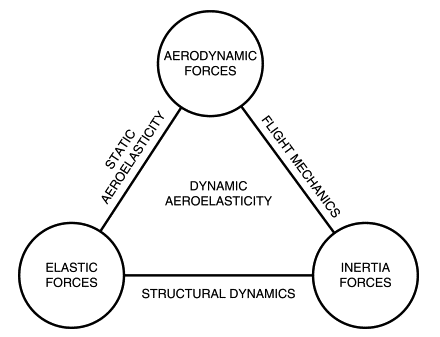
\includegraphics[width=0.5\textwidth]{figs/collar.png}
    \caption{Triângulo de Collar, ilustrando a interação entre 
    as forças aerodinâmicas (A), elásticas (E) e inerciais (I) 
    \cite{Collar1946}.}
    \label{fig:collar}
\end{figure}

\subsection{Formulação Matemática Geral}

A formulação matemática geral de um problema aeroelástico parte da equação do movimento de uma estrutura elástica discretizada pelo Método dos Elementos Finitos (MEF), sujeita a cargas aerodinâmicas inestacionárias. Na forma matricial, esta equação escreve-se como \cite{Hodges2011, Nastran2014}:

\begin{equation}
    \mathbf{M}\ddot{\mathbf{u}} + \mathbf{C}\dot{\mathbf{u}} + 
    \mathbf{K}\mathbf{u} = \mathbf{F}_{aero}(\mathbf{u}, 
    \dot{\mathbf{u}}, t)
    \label{eq:eom_geral}
\end{equation}

\noindent onde $\mathbf{M}$, $\mathbf{C}$ e $\mathbf{K} \in \mathbb{R}^{n \times n}$ são, respetivamente, as matrizes de massa, amortecimento e rigidez globais da estrutura; $\mathbf{u}$, $\dot{\mathbf{u}}$, $\ddot{\mathbf{u}} \in \mathbb{R}^{n}$ são os vetores de deslocamentos, velocidades e acelerações nodais; e $\mathbf{F}_{aero}$ é o vetor de forças aerodinâmicas generalizadas, que depende dos deslocamentos e velocidades estruturais, introduzindo o acoplamento fluido-estrutura \cite{Hodges2011}.

No domínio da frequência, e assumindo escoamento potencial linearizado, as forças aerodinâmicas podem ser expressas em termos da matriz de influência aerodinâmica (\textit{Aerodynamic Influence Coefficient matrix}, AIC) \cite{Roger1977}:

\begin{equation}
    \mathbf{F}_{aero} = q_\infty \mathbf{Q}(ik) \mathbf{u}
    \label{eq:forca_aero}
\end{equation}

\noindent onde $q_\infty = \frac{1}{2}\rho V^2$ é a pressão dinâmica do escoamento livre, $\mathbf{Q}(ik)$ é a matriz AIC avaliada para o número de frequência reduzida $k = \omega b/V$ (com $b$ a semi-corda de referência), e $i$ é a unidade imaginária. Substituindo na Equação \eqref{eq:eom_geral}, obtém-se a equação aeroelástica:

\begin{equation}
    \left[ \mathbf{M}\ddot{\mathbf{u}} + 
    \mathbf{C}\dot{\mathbf{u}} + 
    \mathbf{K}\mathbf{u} \right] - 
    q_\infty \mathbf{Q}(ik)\mathbf{u} = \mathbf{0}
    \label{eq:flutter_eq}
\end{equation}

Esta equação é a base para os métodos de análise de \textit{flutter}, como o método $p$-$k$ e o método $k$, implementados no NX Nastran \cite{Nastran2014}, e justifica a importância central da análise modal como passo preliminar obrigatório de qualquer análise aeroelástica.

\subsection{Classificação dos Fenómenos Aeroelásticos}

A Tabela \ref{tab:fenomenos_aero} resume os principais fenómenos aeroelásticos, a sua natureza, as variáveis estruturais mais relevantes e os métodos de análise tipicamente utilizados.

\begin{table}[H]
\centering
\caption{Classificação dos principais fenómenos aeroelásticos \cite{Wright2015, Dowell2004}.}
\label{tab:fenomenos_aero}
\renewcommand{\arraystretch}{1.8} % Aumentado para dar espaço às quebras de linha
\begin{tabularx}{\textwidth}{
    >{\raggedright\arraybackslash}p{2.4cm} % Largura ideal para quebrar "Inversão de controlos"
    >{\raggedright\arraybackslash}p{1.8cm} % Largura ideal para "Estático/Dinâmico"
    >{\raggedright\arraybackslash}X 
    >{\raggedright\arraybackslash}X
}
\toprule
\textbf{Fenómeno} & \textbf{Tipo} & \textbf{Variáveis estruturais dominantes} & \textbf{Métodos de análise} \\
\midrule
Divergência & Estático & Rigidez torsional $GJ$, posição do centro elástico & Análise de valor próprio estático \\
Inversão de controlos & Estático & Rigidez de flexão e torção, eficácia das superfícies & Análise de equilíbrio aeroelástico estático \\
\textit{Flutter} & Dinâmico & Frequências naturais, amortecimento, acoplamento flexão-torção & Método $p$-$k$; método $k$ \\
Resposta a rajadas & Dinâmico & Frequências naturais, amortecimento modal, massa & Análise espectral; rajadas discretas (1-$\cos$) \\
\textit{Buffeting} & Dinâmico & Frequências naturais, amortecimento aerodinâmico & Análise de resposta em frequência \\
\bottomrule
\end{tabularx}
\end{table}

\subsection{Relevância da Análise Modal no Contexto 
Aeroelástico}

Como se depreende da Equação \eqref{eq:flutter_eq}, a análise aeroelástica dinâmica pressupõe o conhecimento prévio das frequências naturais $\omega_i$ e das formas modais $\boldsymbol{\phi}_i$ da estrutura em vácuo \cite{Craig2006}. Na prática, a equação do movimento é projetada na base modal através da transformação de coordenadas:

\begin{equation}
    \mathbf{u}(t) = \sum_{i=1}^{m} \boldsymbol{\phi}_i \, 
    q_i(t) = \boldsymbol{\Phi} \, \mathbf{q}(t)
    \label{eq:modal_transform}
\end{equation}

\noindent onde $\boldsymbol{\Phi} = [\boldsymbol{\phi}_1 \; \boldsymbol{\phi}_2 \; \cdots \; \boldsymbol{\phi}_m]$ é a matriz modal (com $m \ll n$ modos retidos) e $\mathbf{q}(t)$ é o vetor de coordenadas modais. Substituindo na equação do movimento e pré-multiplicando por $\boldsymbol{\Phi}^T$, obtém-se um sistema de $m$ equações desacopladas, cada uma da forma:

\begin{equation}
    \ddot{q}_i + 2\zeta_i \omega_i \dot{q}_i + 
    \omega_i^2 q_i = \frac{f_i(t)}{m_i}
    \label{eq:modal_eq}
\end{equation}

\noindent onde $\omega_i$ é a frequência natural do modo $i$, $\zeta_i$ é o coeficiente de amortecimento modal, $m_i$ é a massa modal generalizada e $f_i(t)$ é a força aerodinâmica generalizada no modo $i$. Esta projeção modal é o fundamento matemático que justifica a análise modal como pré-requisito da aeroelasticidade \cite{Craig2006}.

\subsection{Requisitos Regulamentares}

O \textit{CS-25.629} da EASA \cite{EASA2022} e o \textit{FAR 25.629} da FAA \cite{FAA2023} estabelecem que a velocidade de \textit{flutter} $V_F$ deve satisfazer:

\begin{equation}
    V_F \geq 1.15 \, V_D
    \label{eq:flutter_margin}
\end{equation}

\noindent onde $V_D$ é a velocidade de projeto em mergulho. Esta margem de 15\% destina-se a acomodar as incertezas associadas à modelação aerodinâmica e estrutural, às variações de configuração de carga e à degradação das propriedades materiais ao longo da vida operacional \cite{Wright2015}. A análise de \textit{flutter} deve ainda ser validada por ensaios de vibração em terra (\textit{Ground Vibration Tests}, GVT), nos quais as frequências naturais e formas modais medidas são comparadas com os resultados do modelo de elementos finitos \cite{Ewins2000}.


\section{Frequências Naturais e Modos de Vibração}
\label{sec:freq_naturais}

A análise das frequências naturais e modos de vibração de uma estrutura constitui o núcleo da dinâmica estrutural e é o ponto de partida indispensável para qualquer estudo aeroelástico. Uma estrutura elástica com $n$ graus de liberdade possui $n$ frequências naturais $\omega_i$ e $n$ modos de vibração associados $\boldsymbol{\phi}_i$, que descrevem completamente o seu comportamento dinâmico livre na ausência de amortecimento e de forças externas \cite{Craig2006, Clough1993}.

\subsection{Problema de Valores e Vetores Próprios}

O ponto de partida formal é a equação do movimento de uma estrutura elástica não amortecida sujeita apenas a forças elásticas e inerciais:

\begin{equation}
    \mathbf{M}\ddot{\mathbf{u}} + \mathbf{K}\mathbf{u} = \mathbf{0}
    \label{eq:eom_livre}
\end{equation}

Assumindo uma solução harmónica da forma $\mathbf{u}(t) = \boldsymbol{\phi} \, e^{i\omega t}$, a substituição na Equação \eqref{eq:eom_livre} conduz ao problema de valores próprios generalizado:

\begin{equation}
    \left( \mathbf{K} - \omega^2 \mathbf{M} \right) 
    \boldsymbol{\phi} = \mathbf{0}
    \label{eq:eigenvalue}
\end{equation}

Para que esta equação admita soluções não triviais, o determinante da matriz do sistema deve ser nulo:

\begin{equation}
    \det\left( \mathbf{K} - \omega^2 \mathbf{M} \right) = 0
    \label{eq:det_zero}
\end{equation}

A Equação \eqref{eq:det_zero} é a \textit{equação característica} do sistema, cujas $n$ raízes reais e não negativas $\omega_1^2 \leq \omega_2^2 \leq \cdots \leq \omega_n^2$ são os \textit{valores próprios} do sistema. As respetivas raízes quadradas $\omega_i$ são as frequências naturais da estrutura, expressas em \si{\radian\per\second}. As frequências naturais em \si{\hertz} obtêm-se por:

\begin{equation}
    f_i = \frac{\omega_i}{2\pi}, \quad i = 1, 2, \ldots, n
    \label{eq:freq_hz}
\end{equation}

A cada frequência natural $\omega_i$ corresponde um vetor próprio $\boldsymbol{\phi}_i \in \mathbb{R}^n$, denominado forma modal ou modo de vibração, que descreve a configuração deformada relativa da estrutura quando vibra na frequência $\omega_i$ \cite{Ewins2000, Maia1997}. As formas modais são determinadas apenas a menos de uma constante de escala arbitrária, sendo habitual normalizá-las segundo um dos seguintes critérios \cite{Craig2006}:

\begin{itemize}
    \item \textbf{Normalização pela massa}: $\boldsymbol{\phi}_i^T \mathbf{M} \boldsymbol{\phi}_i = 1$, convenção adotada por defeito no NX Nastran \cite{Nastran2014};

    \item \textbf{Normalização pelo máximo}: o componente de maior amplitude é normalizado para a unidade, facilitando a interpretação visual das formas modais.
\end{itemize}

\subsection{Propriedades de Ortogonalidade}

Uma propriedade fundamental das formas modais é a \textit{ortogonalidade mútua} relativamente às matrizes $\mathbf{M}$ e $\mathbf{K}$. Para dois modos distintos $i \neq j$ \cite{Clough1993, Inman2014}:

\begin{equation}
    \boldsymbol{\phi}_i^T \mathbf{M} \boldsymbol{\phi}_j = 0, \qquad 
    \boldsymbol{\phi}_i^T \mathbf{K} \boldsymbol{\phi}_j = 0, \qquad i \neq j
    \label{eq:ortogonalidade}
\end{equation}

Para $i = j$, e assumindo normalização pela massa:

\begin{equation}
    \boldsymbol{\phi}_i^T \mathbf{M} \boldsymbol{\phi}_i = m_i = 1, \qquad
    \boldsymbol{\phi}_i^T \mathbf{K} \boldsymbol{\phi}_i = k_i = \omega_i^2
    \label{eq:massas_rigidezes_modais}
\end{equation}

\noindent onde $m_i$ e $k_i$ são a \textit{massa modal generalizada} e a \textit{rigidez modal generalizada} do modo $i$, que permitem definir uma frequência natural equivalente de sistema de um grau de liberdade:

\begin{equation}
    \omega_i = \sqrt{\frac{k_i}{m_i}}
    \label{eq:omega_sdof}
\end{equation}

A ortogonalidade das formas modais é a propriedade que permite desacoplar o sistema de $n$ equações diferenciais acopladas \eqref{eq:eom_livre} em $n$ equações independentes através da transformação modal \eqref{eq:modal_transform}, constituindo o fundamento da \textit{superposição modal} \cite{Craig2006}.

\subsection{Modos de Vibração em Estruturas Alares}

Nas asas de aeronaves, os modos de vibração apresentam características físicas bem definidas que resultam da geometria alar. Os modos fundamentais de uma asa em consola (\textit{cantilever wing}), encastrada na raiz e livre na ponta, são \cite{Bisplinghoff1996, Wright2015}:

\begin{itemize}
    \item \textbf{Flexão} (\textit{bending}): deformação predominantemente fora do plano da asa. O primeiro modo de flexão (1B) é tipicamente o modo de menor frequência, situando-se em aeronaves de grande porte na gama $0.5$--$3$~\si{\hertz} \cite{Megson2012};

    \item \textbf{Torção} (\textit{torsion}): rotação progressiva das secções ao longo da envergadura, alterando o ângulo de ataque local. Este modo é crítico para a divergência e para o \textit{flutter} de flexão-torção;

    \item \textbf{Modos de ordem superior}: modos de flexão e torção com nós intermédios ao longo da envergadura (2B, 3B, 2T, etc.), com frequências crescentes.
\end{itemize}

Para uma asa modelada como viga de Euler-Bernoulli em consola, com rigidez de flexão $EI$ e massa por unidade de comprimento $\mu$ uniformes, a frequência natural do $r$-ésimo modo de flexão é \cite{Rao2011}:

\begin{equation}
    \omega_r = \left(\beta_r L\right)^2 
    \sqrt{\frac{EI}{\mu L^4}}, \qquad r = 1, 2, 3, \ldots
    \label{eq:freq_viga}
\end{equation}

\noindent onde $L$ é a semi-envergadura e $\beta_r L$ são as raízes da equação característica da viga em consola:

\begin{equation}
    \cos(\beta_r L)\cosh(\beta_r L) + 1 = 0
    \label{eq:char_cantilever}
\end{equation}

cujos primeiros valores são $\beta_1 L = 1.8751$, $\beta_2 L = 4.6941$ e $\beta_3 L = 7.8548$ \cite{Rao2011}. De forma análoga, a frequência natural do primeiro modo de torção é \cite{Bisplinghoff1996}:

\begin{equation}
    \omega_{t,1} = \frac{\pi}{2L}
    \sqrt{\frac{GJ}{I_\theta}}
    \label{eq:freq_torcao}
\end{equation}

\noindent onde $GJ$ é a rigidez torsional e $I_\theta$ é a inércia de torção por unidade de comprimento. A separação entre $\omega_{1B}$ e $\omega_{1T}$ é um indicador da margem de \textit{flutter}: quanto mais próximas estiverem estas duas frequências, mais facilmente os modos se acoplam sob ação aerodinâmica, reduzindo a velocidade de \textit{flutter} \cite{Fung1993, Dowell2004}.

\subsection{Métodos Numéricos de Cálculo}

Em estruturas com geometria complexa como a asa do AN-124, o problema de valores próprios \eqref{eq:eigenvalue} é resolvido numericamente após a discretização pelo MEF. No NX Nastran, a análise modal é executada através da solução SOL 103 (\textit{Real Eigenvalue Analysis}), que recorre ao método de Lanczos para a extração dos modos próprios. Este algoritmo iterativo de projeção em subespaço de Krylov calcula exclusivamente os mm valores e vetores próprios de menor magnitude ($m \ll n$), apresentando uma complexidade computacional de $\mathcal{O}(m \cdot n)$ por iteração \cite{Nastran2014, Bathe2014}. Os parâmetros de controlo da análise SOL 103 utilizada neste trabalho são detalhados na Secção \ref{sec:cond_fronteira}.

\section{Análise Modal em Estruturas Aeronáuticas}
\label{sec:analise_modal_aero}

A análise modal consiste na determinação das frequências naturais e das formas modais de uma estrutura. Esta caracterização dinâmica pode ser obtida por via experimental, mediante ensaios de vibração, ou por via numérica, resolvendo o problema de valores próprios associado ao modelo de elementos finitos \cite{Ewins2000, Maia1997}. No contexto aeronáutico, a análise modal assume um papel central no processo de projeto e certificação, uma vez que as frequências naturais e formas modais da estrutura alar determinam, em larga medida, o comportamento aeroelástico da aeronave \cite{Wright2015}.

Uma asa de aeronave é uma estrutura de parede fina (\textit{thin-walled structure}), cujas dimensões de espessura são muito inferiores às dimensões em planta, o que torna os elementos de casca (\textit{shell elements}) a escolha natural e mais eficiente para a sua discretização \cite{Bathe2014, Cook2001}. Esta condição manifesta-se de forma sistemática nos elementos estruturais basilares da asa, nomeadamente no revestimento (\textit{skin}), nas longarinas (\textit{spars}) e nas nervuras (\textit{ribs}). Esta presença transversal fundamenta a escolha metodológica adotada no presente estudo.

\subsection{Elementos CQUAD8}

No presente trabalho, a discretização da asa foi realizada com elementos do tipo CQUAD8, disponíveis no NX Nastran. O CQUAD8 é um elemento de casca quadrilateral isoparamétrico de segunda ordem, constituído por 8 nós, dos quais 4 se localizam nos vértices e 4 nos pontos médios das arestas. Cada nó dispõe de 6 graus de liberdade, correspondentes a 3 translações e 3 rotações, o que perfaz um total de 48 graus de liberdade por elemento \cite{Nastran2014, Cook2001}. As principais vantagens deste elemento relativamente ao elemento de primeira ordem CQUAD4 são a maior precisão na representação de campos de deformação com gradientes acentuados, a melhor aproximação de geometrias curvas como o perfil aerodinâmico TsAGI, e a convergência mais rápida para a solução exacta para o mesmo número de graus de liberdade \cite{Bathe2014, Zienkiewicz2005}. A integração numérica é realizada por quadratura de Gauss-Legendre com esquema $3 \times 3$ pontos no plano do elemento, com integração ao longo da espessura segundo a teoria de Mindlin-Reissner, que incorpora os efeitos de deformação por corte transversal \cite{Nastran2014}.

\subsection{Materiais}

O modelo numérico da asa recorre a dois materiais distintos, selecionados de forma a aproximar as propriedades das ligas estruturais típicas de aeronaves de grande porte:

\begin{itemize}
    \item \textbf{Liga de alumínio 2024-T3}: utilizada no revestimento (\textit{skin}) da asa, amplamente utilizada em estruturas aeronáuticas primárias sujeitas a cargas de fadiga, devido à sua elevada resistência à propagação de fissuras (\textit{damage tolerance}) \cite{Megson2012, ASM2008};

    \item \textbf{Liga de alumínio 7075-T6}: utilizada nas longarinas (\textit{spars}) e nervuras (\textit{ribs}), sendo preferida em elementos estruturais sujeitos a elevadas tensões de compressão e corte \cite{Megson2012, ASM2008}.
\end{itemize}

As propriedades mecânicas de ambas as ligas são apresentadas na Tabela \ref{tab:materiais}. Do ponto de vista da análise modal, as propriedades determinantes são o módulo de Young $E$ e a massa volúmica $\rho$. As duas ligas apresentam valores muito próximos destas propriedades, pelo que a distinção de material entre componentes tem impacto reduzido sobre as frequências naturais absolutas, sendo contudo importante para a representatividade física do modelo \cite{Megson2012}.

\begin{table}[H]
\centering
\caption{Propriedades mecânicas das ligas de alumínio 
utilizadas na modelação \cite{ASM2008}.}
\label{tab:materiais}
\renewcommand{\arraystretch}{1.4}
\begin{tabularx}{\textwidth}{p{4.5cm} X X}
\toprule
\textbf{Propriedade} & \textbf{Al 2024-T3} & 
\textbf{Al 7075-T6} \\
\midrule
Módulo de Young ($E$)
    & \SI{73.1}{\giga\pascal}
    & \SI{71.7}{\giga\pascal} \\
Coeficiente de Poisson ($\nu$)
    & $0.33$
    & $0.33$ \\
Módulo de corte ($G$)
    & \SI{28.0}{\giga\pascal}
    & \SI{26.9}{\giga\pascal} \\
Massa volúmica ($\rho$)
    & \SI{2780}{\kilo\gram\per\cubic\meter}
    & \SI{2810}{\kilo\gram\per\cubic\meter} \\
Tensão de cedência ($\sigma_y$)
    & \SI{345}{\mega\pascal}
    & \SI{503}{\mega\pascal} \\
Tensão de rotura ($\sigma_u$)
    & \SI{483}{\mega\pascal}
    & \SI{572}{\mega\pascal} \\
Componentes
    & \textit{Skin}
    & \textit{Spars} e \textit{Ribs} \\
\bottomrule
\end{tabularx}
\end{table}

\subsection{Número de Modos Calculados}

Foram calculados os primeiros 10 modos de vibração da estrutura alar em cada configuração, utilizando o solver de Lanczos do NX Nastran (SOL 103) \cite{Nastran2014}. Esta escolha justifica-se pelo facto de os modos de menor frequência serem os que mais contribuem para a resposta dinâmica da estrutura e os que apresentam maior relevância aeroelástica \cite{Craig2006}. Em particular, os primeiros modos de flexão e de torção são os que determinam a velocidade de \textit{flutter} e a velocidade de divergência da asa \cite{Bisplinghoff1996, Fung1993}.

A massa modal acumulada dos primeiros $m$ modos (\textit{Effective Modal Mass fraction}, EMFA), definida como:

\begin{equation}
    \text{EMFA} = \sum_{r=1}^{m} 
    \frac{\left( \boldsymbol{\phi}_r^T \mathbf{M} 
    \mathbf{1} \right)^2}{M_{total}}
    \label{eq:emf}
\end{equation}

\noindent é um indicador da completude da base modal utilizada. Em geral, recomenda-se EMFA $> 90\%$ para garantir que a resposta dinâmica está adequadamente representada \cite{Craig2006, Nastran2014}.

\section{Influência dos Parâmetros Geométricos nas 
Frequências Naturais}
\label{sec:efeitos_geometricos}

A geometria de uma asa de aeronave é um dos fatores que mais diretamente condiciona as suas frequências naturais e formas modais. Através das expressões analíticas desenvolvidas na Secção \ref{sec:freq_naturais}, é possível identificar os parâmetros geométricos com maior influência sobre o comportamento dinâmico da estrutura alar e, consequentemente, sobre o seu comportamento aeroelástico \cite{Bisplinghoff1996, Wright2015}.

\subsection{Ângulo de Enflechamento}
\label{sec:sweep}

O ângulo de enflechamento (\textit{sweep angle}) $\Lambda$ define a inclinação do bordo de ataque relativamente à direção perpendicular ao eixo longitudinal da aeronave. No modelo estudado, $\Lambda = \ang{25}$, valor representativo do enflechamento da asa do Antonov AN-124 \cite{Antonov2004}.

O enflechamento influencia significativamente o acoplamento entre os modos de flexão e de torção. Para uma asa enflechada, a deflexão vertical induz uma componente de torção, e vice-versa, devido à rotação do eixo elástico relativamente à direção de voo \cite{Dowell2004}. Este acoplamento pode ser quantificado através da matriz de rigidez de uma secção alar enflechada \cite{Hodges2011}:

\begin{equation}
    \begin{Bmatrix} M_b \\ M_t \end{Bmatrix} =
    \begin{bmatrix} 
        EI & EI\tan\Lambda \\ 
        EI\tan\Lambda & GJ + EI\tan^2\Lambda 
    \end{bmatrix}
    \begin{Bmatrix} \kappa_b \\ \kappa_t 
    \end{Bmatrix}
    \label{eq:rigidez_enflechamento}
\end{equation}

\noindent onde $M_b$ e $M_t$ são os momentos de flexão e torção, $\kappa_b$ e $\kappa_t$ são as curvaturas de flexão e torção, e o termo $EI\tan\Lambda$ representa o acoplamento induzido pelo enflechamento. Para $\Lambda = \ang{25}$, $\tan\Lambda \approx 0.466$, representando um acoplamento não negligenciável \cite{Bisplinghoff1996}. Como consequência, as formas modais de uma asa enflechada são modos mistos (\textit{coupled bending-torsion modes}), com frequências naturais que diferem das previstas pelas expressões analíticas para viga reta \eqref{eq:freq_viga} e \eqref{eq:freq_torcao} \cite{Wright2015}.

\subsection{Razão de Afilamento}

A razão de afilamento (\textit{taper ratio}) é definida como o quociente entre a corda na ponta e a corda na raiz:

\begin{equation}
    \lambda = \frac{c_{tip}}{c_{root}} = 
    \frac{700}{2000} = 0.35
    \label{eq:taper_ratio}
\end{equation}

Este valor é representativo de asas de aeronaves de transporte de grande porte, situando-se na gama típica $0.2 \leq \lambda \leq 0.5$ \cite{Raymer2018}. A corda local varia linearmente com a posição ao longo da envergadura:

\begin{equation}
    c(y) = c_{root}\left(1 - 
    \frac{1-\lambda}{L}y\right), \qquad 0 \leq y \leq L
    \label{eq:corda_local}
\end{equation}

A rigidez de flexão local é aproximadamente proporcional ao cubo da corda local \cite{Megson2012}:

\begin{equation}
    EI(y) \propto c(y)^3
    \label{eq:EI_local}
\end{equation}

Esta variação de rigidez ao longo da envergadura concentra as deformações modais nas regiões de menor rigidez, geralmente na ponta da asa, e resulta em frequências naturais mais elevadas em comparação com as de uma asa de corda constante com idêntico comprimento e material \cite{Rao2011}.

\subsection{Posição e Orientação das Nervuras}

As nervuras (\textit{ribs}) são elementos estruturais transversais que desempenham um papel fundamental na estrutura alar: mantêm a forma do perfil aerodinâmico, transmitem as cargas aerodinâmicas às longarinas, estabilizam o revestimento contra encurvadura e contribuem para a rigidez torsional da caixa alar \cite{Megson2012, Niu1988}. Do ponto de vista da dinâmica estrutural, as nervuras influenciam as frequências naturais através de dois mecanismos:

\begin{itemize}
    \item \textbf{Contribuição para a rigidez}: aumentam a rigidez local da secção transversal, em particular a rigidez torsional. A sua contribuição depende da orientação, espessura, espaçamento e condições de ligação \cite{Niu1988};

    \item \textbf{Contribuição para a massa}: adicionam massa distribuída ao longo da envergadura, reduzindo as frequências naturais e influenciando a forma dos modos \cite{Craig2006}.
\end{itemize}

A orientação das nervuras relativamente ao eixo da fuselagem é a variável de estudo central deste trabalho, conforme descrito no Capítulo \ref{chap:variavel}. A sua influência sobre a rigidez torsional da caixa alar pode ser compreendida recorrendo à teoria de Bredt para secções de parede fina fechadas \cite{Megson2012}:

\begin{equation}
    GJ_{eff} = \frac{4A_{cell}^2}{\oint \frac{ds}{Gt(s)}}
    \label{eq:bredt}
\end{equation}

\noindent onde $A_{cell}$ é a área da secção transversal da caixa alar e $t(s)$ é a espessura do painel ao longo do contorno $s$. Nervuras perpendiculares ao bordo de ataque (Configuração A) são mais eficientes na resistência às tensões de corte induzidas pela torção, uma vez que estão alinhadas com as trajetórias de fluxo de corte naturais da caixa alar enflechada \cite{Niu1988, Megson2012}.

\subsection{Síntese dos Efeitos Geométricos}

A Tabela \ref{tab:efeitos_geometricos} sintetiza a influência qualitativa dos principais parâmetros geométricos sobre as frequências naturais dos modos de flexão e torção.

\begin{table}[H]
\centering
\caption{Influência qualitativa dos parâmetros geométricos sobre as frequências naturais da asa \cite{Wright2015, Megson2012, Bisplinghoff1996}.}
\label{tab:efeitos_geometricos}
\renewcommand{\arraystretch}{1.5}
\begin{tabularx}{\textwidth}{l >{\raggedright\arraybackslash}X >{\raggedright\arraybackslash}X}
\toprule
\textbf{Parâmetro} & \textbf{Efeito sobre $f_{\text{flexão}}$} & \textbf{Efeito sobre $f_{\text{torção}}$} \\
\midrule
$\uparrow$ Envergadura $L$           & $\downarrow$ (proporcional a $1/L^2$) & $\downarrow$ (proporcional a $1/L$) \\
$\uparrow$ Espessura \textit{skin} $t_s$ & $\uparrow$ (rigidez e massa)          & $\uparrow$ (rigidez torsional) \\
$\uparrow$ Afilamento $\lambda$      & $\uparrow$ (menos massa na ponta)     & $\uparrow$ (menos massa na ponta) \\
$\uparrow$ Enflechamento $\Lambda$   & Acoplamento flexão-torção             & Acoplamento flexão-torção \\
Orientação dos \textit{ribs}         & Efeito secundário sobre $EI$          & Efeito primário sobre $GJ_{eff}$ \\
$\uparrow$ Nº de \textit{ribs}       & $\uparrow$ (massa e rigidez locais)   & $\uparrow$ (rigidez torsional) \\
\bottomrule
\end{tabularx}
\end{table}

% SUBSTITUIR o último parágrafo da Secção 2.4 por:

A última linha da Tabela \ref{tab:efeitos_geometricos} assume particular relevância: a orientação das nervuras exerce influência preponderante sobre $GJ_{eff}$ e efeito secundário sobre $EI$, o que sugere que as diferenças entre configurações se manifestarão com maior intensidade nas frequências dos modos de torção do que nos modos de flexão. Contudo, esta projeção teórica pressupõe que a orientação constitui a única variável diferenciadora, condição que não se verifica integralmente neste estudo. As duas configurações divergem igualmente no número de nervuras (13 face a 10) e no respetivo espaçamento, fatores que alteram a distribuição local de massa e rigidez e que podem sobrepor-se ao efeito da orientação. A validação ou refutação desta hipótese será analisada à luz dos resultados numéricos apresentados no Capítulo \ref{chap:resultados}.

\chapter{O Avião Antonov AN-124}
\label{chap:an124}

\section{Descrição Geral e Características}

O Antonov AN-124 \textit{Ruslan} é uma aeronave de transporte estratégico pesado de grande porte, desenvolvida pelo Bureau de Projeto Antonov na então União Soviética, com o seu primeiro voo a ocorrer em 26 de dezembro de 1982 \cite{Gordon2008}. Foi concebida para o transporte de equipamentos de grande dimensão e peso, tendo posteriormente encontrado vasta aplicação no mercado civil de carga aérea pesada, onde continua a ser uma das aeronaves com maior capacidade de carga do mundo \cite{GarciaFernandez2025}. As principais características gerais da aeronave são apresentadas na Tabela \ref{tab:an124_specs}.

\begin{table}[H]
\centering
\caption{Características gerais do Antonov AN-124-100 
\cite{Gordon2008, GarciaFernandez2025}.}
\label{tab:an124_specs}
\renewcommand{\arraystretch}{1.4}
\begin{tabularx}{\textwidth}{p{5.5cm} X}
\toprule
\textbf{Parâmetro} & \textbf{Valor} \\
\midrule
Comprimento total           & \SI{69.1}{\meter} \\
Envergadura total           & \SI{73.3}{\meter} \\
Altura                      & \SI{21.1}{\meter} \\
Área alar                   & \SI{628}{\meter\squared} \\
Peso máximo à descolagem    & \SI{405000}{\kilo\gram} \\
Carga útil máxima           & \SI{150000}{\kilo\gram} \\
Velocidade de cruzeiro      & \SI{865}{\kilo\meter\per\hour} \\
Altitude de cruzeiro        & \SI{12000}{\meter} \\
Alcance (com carga máxima)  & \SI{5400}{\kilo\meter} \\
Motorização                 & 4 $\times$ ZMKB Progress D-18T \\
Empuxo por motor            & \SI{229.5}{\kilo\newton} \\
\bottomrule
\end{tabularx}
\end{table}

% FIGURA: Vista geral do Antonov AN-124
\begin{figure}[H]
    \centering
    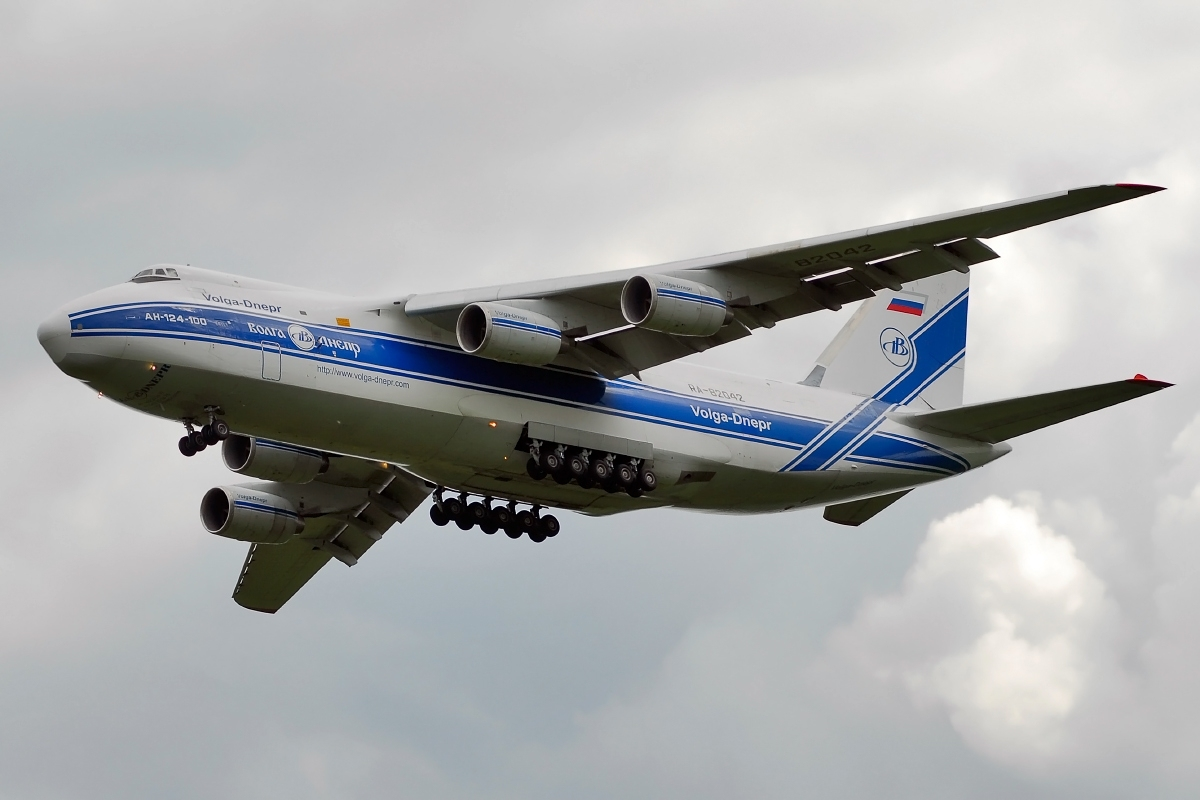
\includegraphics[width=0.6\textwidth]{figs/an124_geral.jpg}
    \caption{Vista geral do Antonov AN-124 \textit{Ruslan} 
    \cite{Gordon2008}.}
    \label{fig:an124_geral}
\end{figure}

\section{Geometria e Estrutura da Asa}

A asa do AN-124 caracteriza-se por uma geometria trapezoidal em planta, com enflechamento do bordo de ataque de $\Lambda = \ang{25}$. O perfil aerodinâmico adotado pertence à família TsAGI, com 12\% de espessura relativa (Figura \ref{fig:perfil_asa}), tendo sido desenvolvido pelo Instituto Central de Aerodinâmica e Hidrodinâmica (\textit{Tsentralny Aerogidrodinamichesky Institut}, TsAGI) da antiga União Soviética \cite{Gordon2008, GarciaFernandez2025}. O perfil TsAGI é simétrico e a asa não apresenta torção geométrica (\textit{washout}), mantendo o plano médio do perfil constante ao longo de toda a envergadura. As principais características geométricas são apresentadas na Tabela \ref{tab:asa_specs}. Devido à natureza militar da aeronave e consecutivas reduzida divulgação de especificações, não existem disponíveis plantas da asa real do avião. Contudo no projeto de licenciatura de \citet{GarciaFernandez2025} um modelo real foi desenvolvido a uma escala de 1:50, encontrando-se a planta do avião na Figura \ref{fig:an124_asa_planta}. 

\begin{figure}[H]
    \centering
    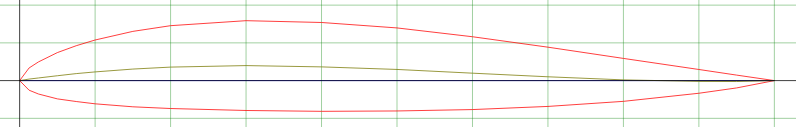
\includegraphics[width=0.85\textwidth]{figs/perfil_asa.png}
    \caption{Perfil TsAGI 12%
    \cite{AirfoilTools}.}
    \label{fig:perfil_asa}
\end{figure}

\begin{table}[H]
\centering
\caption{Características geométricas da asa do Antonov 
AN-124 \cite{GarciaFernandez2025, Gordon2008}.}
\label{tab:asa_specs}
\renewcommand{\arraystretch}{1.4}
\begin{tabularx}{\textwidth}{p{5.5cm} X}
\toprule
\textbf{Parâmetro} & \textbf{Valor} \\
\midrule
Envergadura total               & \SI{73.3}{\meter} \\
Semi-envergadura                & \SI{36.65}{\meter} \\
Corda na raiz                   & \SI{10.0}{\meter} \\
Corda na ponta                  & \SI{3.5}{\meter} \\
Razão de afilamento $\lambda$   & $0.35$ \\
Ângulo de enflechamento $\Lambda$ & $\ang{25}$ \\
Alongamento (\textit{aspect ratio}) $AR$ & $8.57$ \\
Perfil aerodinâmico             & TsAGI 12\% \\
Torção geométrica               & Nenhuma \\
\bottomrule
\end{tabularx}
\end{table}

% FIGURA: Planta da asa do AN-124 com dimensões principais
\begin{figure}[H]
    \centering
    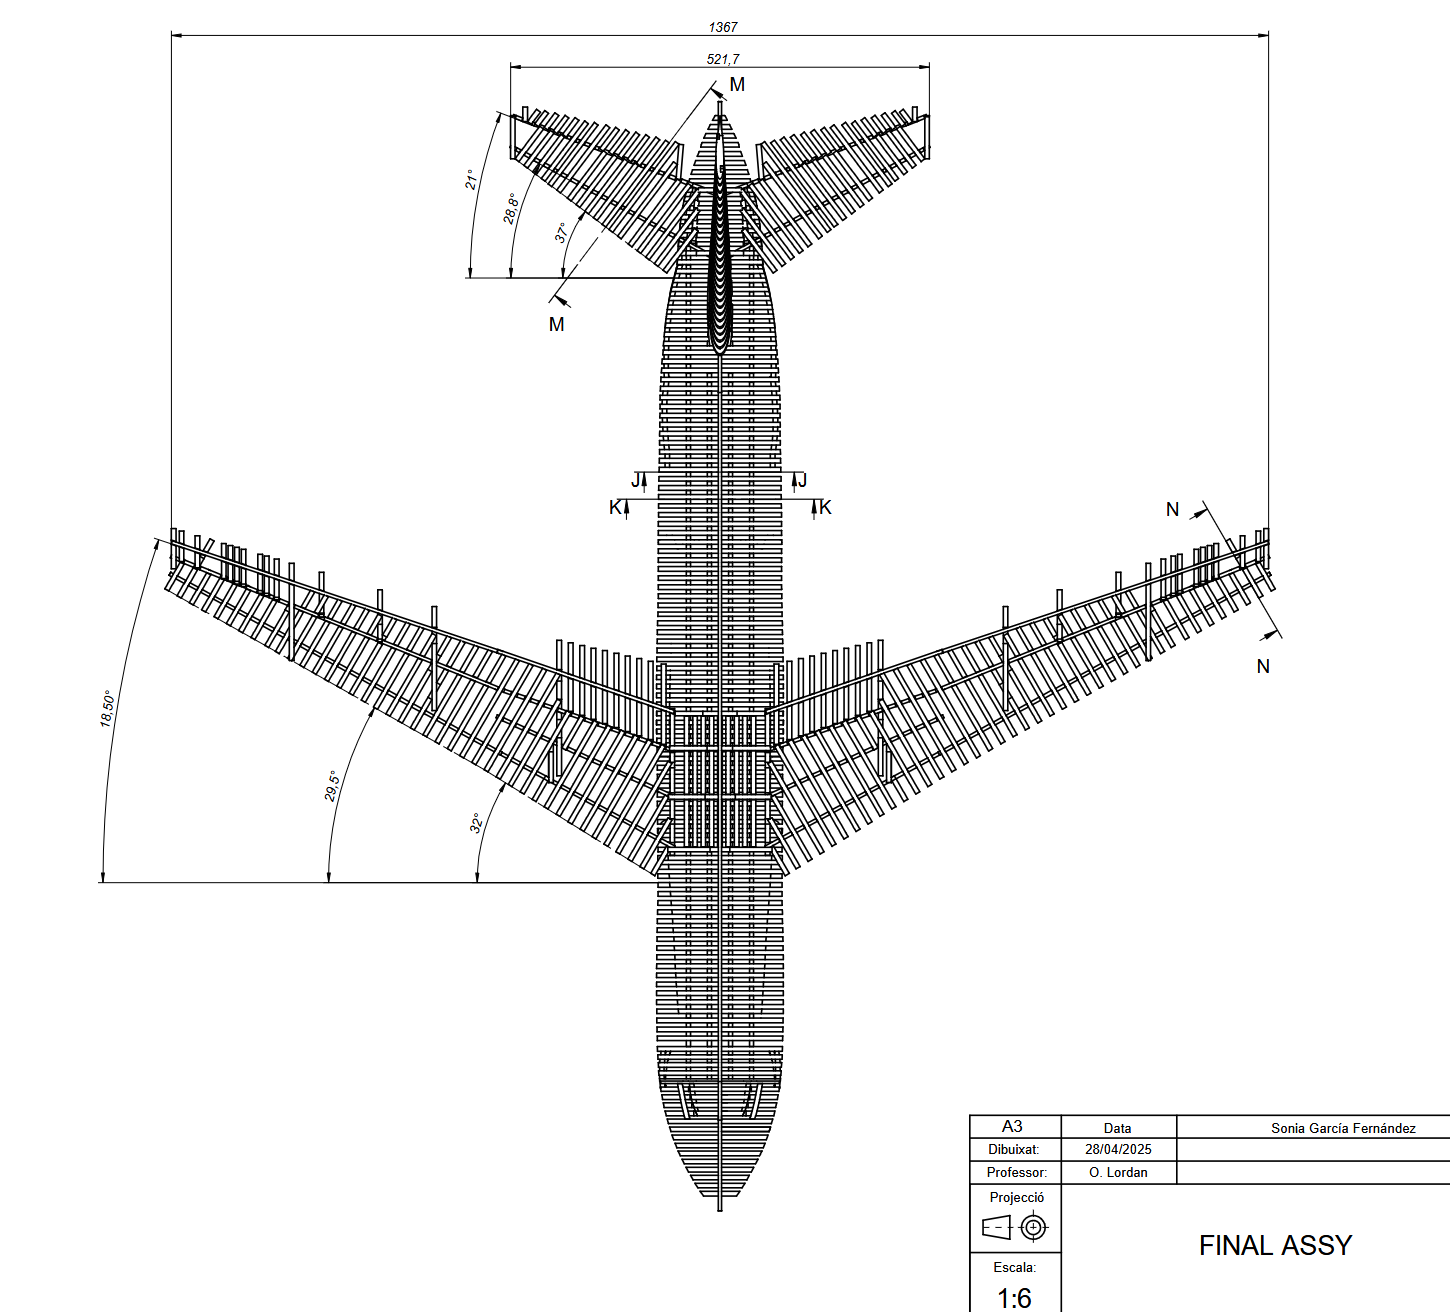
\includegraphics[width=0.6\textwidth]{figs/an124_asa_planta.png}
    \caption{Planta da asa do Antonov AN-124 com as principais 
    dimensões geométricas \cite{GarciaFernandez2025}.}
    \label{fig:an124_asa_planta}
\end{figure}

O alongamento da asa, definido como $AR = b^2/S = 73.3^2/628 \approx 8.57$, é um valor moderado para uma aeronave de transporte pesado, refletindo o compromisso entre eficiência aerodinâmica e rigidez estrutural alar \cite{Raymer2018}. A estrutura interna da asa segue a filosofia construtiva clássica das aeronaves de transporte de grande porte, baseada numa caixa alar (\textit{wing box}) constituída por longarinas, nervuras e revestimento, sendo estes componentes descritos em detalhe no Capítulo \ref{chap:modelacao} \cite{Niu1988, Megson2012}.

\section{Dados Estruturais Relevantes para a Modelação}

Para efeitos de modelação numérica, a geometria real da asa foi sujeita a um conjunto de simplificações e adaptações descritas em detalhe no Capítulo \ref{chap:modelacao}. A Tabela \ref{tab:modelo_vs_real} apresenta a comparação entre as dimensões da asa real e as do modelo numérico, evidenciando as principais diferenças introduzidas pela redução de escala.

\begin{table}[H]
\centering
\caption{Comparação entre a geometria da asa real do AN-124 e o modelo numérico utilizado neste trabalho.}
\label{tab:modelo_vs_real}
\renewcommand{\arraystretch}{1.4}
% Ajustamos o peso das colunas X: 0.8 para a segunda e 1.2 para a terceira
\begin{tabularx}{\textwidth}{l >{\hsize=0.8\hsize\raggedright\arraybackslash}X >{\hsize=1.2\hsize\raggedright\arraybackslash}X}
\toprule
\textbf{Parâmetro} & \textbf{Asa real} & \textbf{Modelo numérico} \\
\midrule
Semi-envergadura & \SI{36.65}{\meter} & \SI{4.0}{\meter} \\
Corda na raiz & \SI{10.0}{\meter} & \SI{2.0}{\meter} \\
Corda na ponta & \SI{3.5}{\meter} & \SI{0.7}{\meter} \\
Razão de afilamento & $0.35$ & $0.35$ \\
Ângulo de enflechamento & $\ang{25}$ & $\ang{25}$ \\
Perfil aerodinâmico & TsAGI 12\% & TsAGI 12\% \\
Torção geométrica & Nenhuma & Nenhuma \\
Material & Ligas Al série 2000/7000 & Al 2024-T3 (\textit{skin}), Al 7075-T6 (\textit{spars} e \textit{ribs}) \\
Escala & 1:1 & $\approx$ 1:9 \\
\bottomrule
\end{tabularx}
\end{table}

A redução de escala foi aplicada de forma proporcional a todas as dimensões lineares, preservando a razão de afilamento, o ângulo de enflechamento e as relações geométricas relativas entre os componentes estruturais. Para estruturas geometricamente semelhantes com o mesmo material, a frequência natural escala inversamente com a dimensão linear característica \cite{Craig2006}:

\begin{equation}
    \frac{f_{modelo}}{f_{real}} = 
    \frac{L_{real}}{L_{modelo}} \approx 
    \frac{36.65}{4.0} \approx 9.16
    \label{eq:escala_freq}
\end{equation}

As frequências naturais do modelo são assim aproximadamente 9 vezes superiores às da asa real. Esta diferença é expectável e não compromete a validade do estudo comparativo entre as duas configurações de nervuras, uma vez que o objetivo é avaliar a influência \textit{relativa} da orientação das nervuras sobre as frequências naturais e formas modais, e não reproduzir os valores absolutos da aeronave real \cite{Dowell2004}.

\chapter{Modelação da Asa}
\label{chap:modelacao}

\section{Simplificações e Hipóteses de Modelação}
\label{sec:simplificacoes}

A modelação numérica de uma estrutura aeronáutica de grande porte envolve inevitavelmente um conjunto de simplificações que visam equilibrar a fidelidade física do modelo com a viabilidade computacional da análise. No presente trabalho, as simplificações introduzidas justificam-se pelo escopo comparativo da investigação, que visa confrontar o comportamento modal de duas configurações de nervuras, e não pela pretensão de replicar com exatidão a resposta estrutural da aeronave em condições reais \cite{Dowell2004}. As principais simplificações adotadas são as seguintes:

\begin{itemize}
    \item \textbf{Redução de escala}: a semi-envergadura foi reduzida de \SI{36.65}{\meter} para \SI{4.0}{\meter}, mantendo todas as relações geométricas relativas constantes, conforme discutido no Capítulo \ref{chap:an124};

    \item \textbf{Discretização com elementos de casca 2D}: toda a estrutura foi modelada com elementos CQUAD8, cuja formulação e adequação foram descritas na Secção \ref{sec:analise_modal_aero};

    \item \textbf{Corte do bordo de fuga}: a zona do bordo de fuga foi truncada a \SI{45}{\milli\meter} do bordo de fuga real e a secção resultante foi fechada com um painel plano. Esta simplificação evita elementos de malha com elevada razão de aspeto na zona de espessura muito reduzida do perfil TsAGI, sem impacto significativo na rigidez e massa globais \cite{Bathe2014};
    
    \item \textbf{Corte da nervura final na Configuração A}: na Configuração A, a nervura de ponta inclinada a 25° gerava uma interseção geometricamente complexa com o bordo de ataque, originando problemas de densidade e continuidade da malha nessa zona. Para resolver esta situação, a zona de interseção foi cortada, eliminando a região problemática sem impacto significativo nos resultados modais, uma vez que se trata de uma zona de pequena dimensão e reduzida contribuição para a rigidez e massa globais \cite{Bathe2014};

    \item \textbf{Ausência de elementos de ligação}: a conectividade entre nervuras, longarinas e revestimento é garantida pela partilha de nós entre elementos adjacentes (ligação rígida implícita), não sendo modelados os elementos de ligação reais (rebites, cantoneiras). Esta simplificação é comum em modelos de análise modal global \cite{Wright2015};

    \item \textbf{Ausência de massa não estrutural}: a massa de combustível, sistemas e equipamentos não foi incluída, tendendo a sobrestimar as frequências naturais relativamente à aeronave real \cite{Craig2006};

    \item \textbf{Encastramento na raiz}: a ligação asa-fuselagem foi modelada como encastramento perfeito, ignorando a flexibilidade da fuselagem e da junta estrutural, o que sobrestima ligeiramente as frequências naturais \cite{Hodges2011}.
\end{itemize}

\section{Definição da Geometria}

\subsection{Processo de Modelação}

A geometria da asa, ilustrada na Figura \ref{fig:asa_sw}, foi desenvolvida em \textit{SolidWorks} a partir das dimensões reais do Antonov AN-124, escaladas para o modelo reduzido, e subsequentemente importada para o  NX Siemens para geração da malha de elementos finitos e realização da análise modal. O processo de modelação seguiu a seguinte sequência:

\begin{enumerate}
    \item Definição do perfil aerodinâmico TsAGI 12\% nas secções de raiz e ponta, com cordas de \SI{2000}{\milli\meter} e \SI{700}{\milli\meter}, respetivamente;

    \item Geração da superfície do revestimento por interpolação entre os dois perfis, com aplicação do ângulo de enflechamento de $\ang{25}$;

    \item Definição das longarinas dianteira e traseira como superfícies planas interiores à caixa alar;

    \item Truncagem do bordo de fuga a \SI{45}{\milli\meter} e fecho da secção com um painel plano;

    \item Definição das nervuras nas duas configurações estudadas, conforme descrito no Capítulo \ref{chap:variavel};

    \item Importação da geometria para o NX Siemens e conversão das superfícies em entidades de elementos finitos.
\end{enumerate}


\begin{figure}[H]
    \centering
    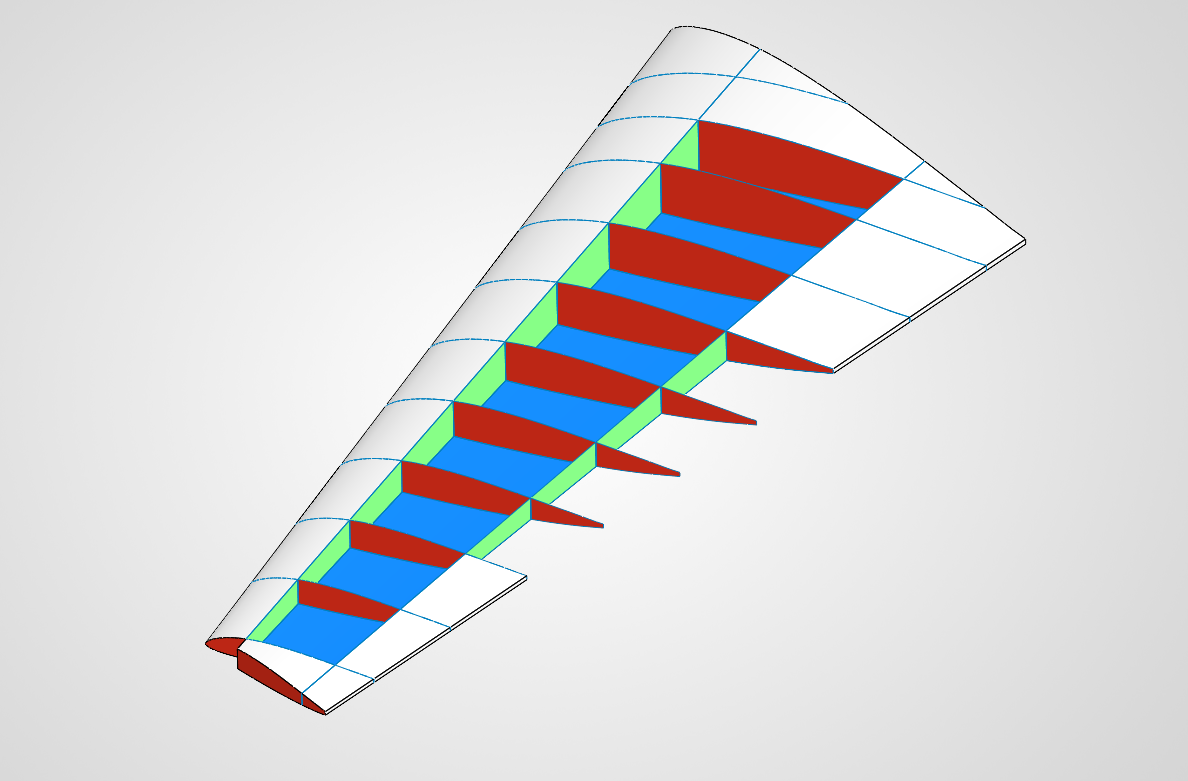
\includegraphics[width=0.85\textwidth]{figs/asa_sw.png}
    \caption{Vista da estrutura interna da asa modelada no SolidWorks, na qual é possível observar a \textit{skin} (azul), as \textit{spars} (verde) e a \textit{ribs} (vermelho). A parte superior da foi \textit{skin} omitida para permitir a visualização da estrutura interna.}
    \label{fig:asa_sw}
\end{figure}


\subsection{Geometria da Caixa Alar}

A caixa alar é definida pelos parâmetros geométricos apresentados na Tabela \ref{tab:geom_caixa_alar}. A spar dianteira está posicionada a 25\% da corda local e a spar traseira a 70\% da corda local, definindo uma caixa alar com largura de 45\% da corda, constante ao longo da envergadura \cite{Niu1988}.

\begin{table}[H]
\centering
\caption{Dimensões geométricas principais do modelo da asa.}
\label{tab:geom_caixa_alar}
\renewcommand{\arraystretch}{1.4}
\begin{tabularx}{\textwidth}{p{5.5cm} X}
\toprule
\textbf{Parâmetro} & \textbf{Valor} \\
\midrule
Semi-envergadura                    
    & \SI{4000}{\milli\meter} \\
Corda na raiz                       
    & \SI{2000}{\milli\meter} \\
Corda na ponta                      
    & \SI{700}{\milli\meter} \\
Razão de afilamento $\lambda$       
    & $0.35$ \\
Ângulo de enflechamento $\Lambda$   
    & $\ang{25}$ \\
Posição da spar dianteira           
    & \SI{500}{\milli\meter} do bordo de ataque (25\% da corda) \\
Posição da spar traseira            
    & \SI{600}{\milli\meter} do bordo de fuga (70\% da corda) \\
Corte do bordo de fuga              
    & \SI{45}{\milli\meter} do bordo de fuga \\
Espessura da \textit{skin}          
    & \SI{2}{\milli\meter} \\
Espessura das \textit{spars}            
    & \SI{4}{\milli\meter} \\
Espessura das \textit{ribs}              
    & \SI{2.3}{\milli\meter} \\
\bottomrule
\end{tabularx}
\end{table}

\section{Materiais e Propriedades Estruturais}

Os materiais utilizados na modelação foram descritos em detalhe na Secção \ref{sec:analise_modal_aero}, onde as suas propriedades mecânicas são apresentadas na Tabela \ref{tab:materiais}. A atribuição de materiais a cada componente estrutural é resumida na Tabela \ref{tab:material_componentes}.

\begin{table}[H]
\centering
\caption{Atribuição de materiais e espessuras aos 
componentes estruturais do modelo.}
\label{tab:material_componentes}
\renewcommand{\arraystretch}{1.4}
\begin{tabularx}{\textwidth}{l l l >{\raggedright\arraybackslash}X}
\toprule
\textbf{Componente} & \textbf{Material} & \textbf{Espessura} & \textbf{Função estrutural} \\
\midrule
\textit{Skin}  & Al 2024-T3 & \SI{2}{\milli\meter}   & Resistência à torção e cargas de membrana \\
\textit{Spars} & Al 7075-T6 & \SI{4}{\milli\meter}   & Resistência ao momento fletor e corte \\
\textit{Ribs}  & Al 7075-T6 & \SI{2.3}{\milli\meter} & Manutenção do perfil e transmissão de cargas \\
\bottomrule
\end{tabularx}
\end{table}


No NX Nastran, as propriedades de cada material são definidas através de cartões MAT1 (material isotrópico linear elástico), e as espessuras dos elementos de casca através de cartões PSHELL \cite{Nastran2014}.

\section{Malha de Elementos Finitos e Condições de 
Fronteira}
\label{sec:cond_fronteira}

\subsection{Malha de Elementos Finitos}

A malha, representada na Figura \ref{fig:malha_nx}, foi gerada no NX Siemens utilizando exclusivamente elementos CQUAD8, descritos na Secção \ref{sec:analise_modal_aero}. A qualidade da malha foi verificada através dos critérios disponíveis no NX Siemens, nomeadamente a razão de aspeto, o ângulo interno mínimo e máximo, e o critério de distorção de Jacobiano. Elementos com razão de aspeto superior a 5 ou com ângulos internos fora do intervalo $[\ang{45}, \ang{135}]$ foram identificados e corrigidos \cite{Bathe2014, Cook2001}.


\begin{figure}[H]
    \centering
    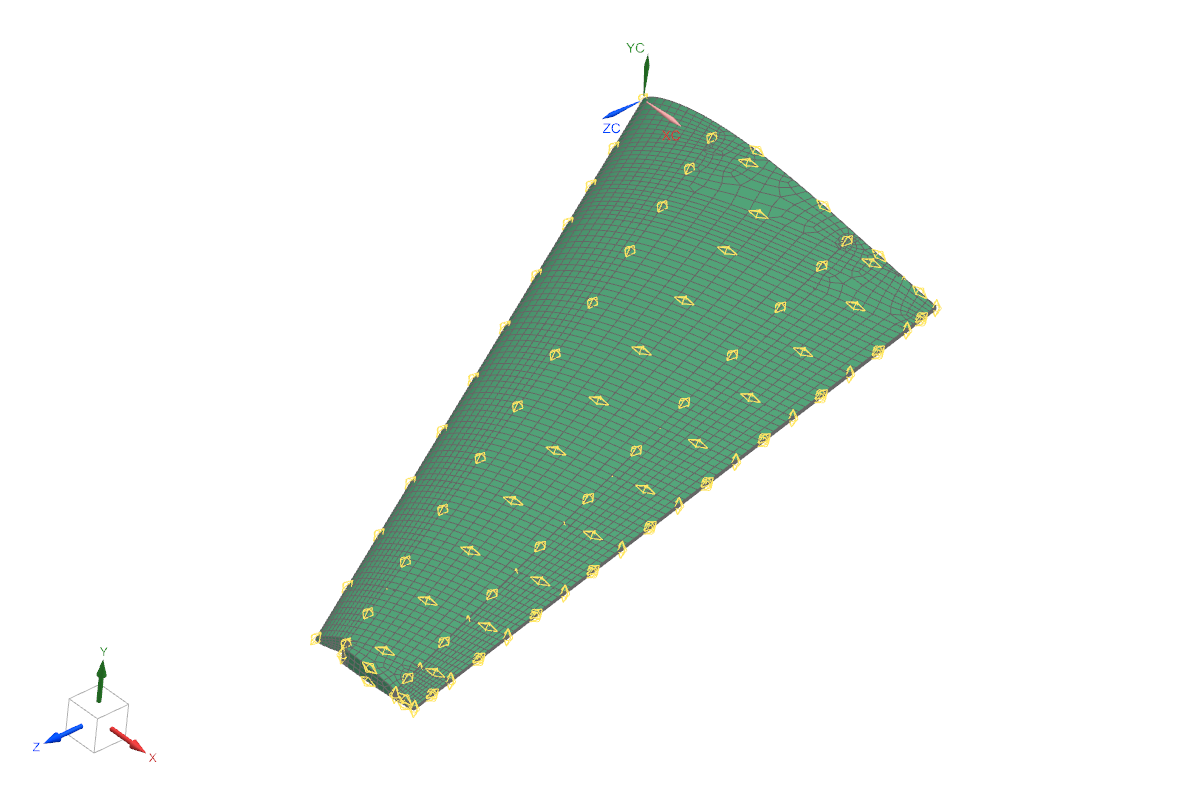
\includegraphics[width=0.85\textwidth]{figs/malha_nx.png}
    \caption{Vista da malha de elementos finitos CQUAD8 gerada no NX Siemens. A configuração de nervuras representada é detalhada no Capítulo \ref{chap:variavel}. As zonas a amarelo representam a aplicação dos \textit{Mesh Controls} descritos posteriormente na secção \ref{subsub:mesh control}}
    \label{fig:malha_nx}
\end{figure}

\subsubsection{Controlo da Malha e Continuidade} \label{subsub:mesh control}

A geração automática da malha em superfícies de geometria complexa, como as interseções entre o revestimento, as longarinas e as nervuras, pode originar descontinuidades nodais nas zonas de fronteira entre componentes adjacentes. Para garantir a continuidade da malha em toda a estrutura, foi necessário recorrer a três procedimentos adicionais no NX Siemens:

\begin{itemize}
    \item \textbf{\textit{Mesh Controls}}: foram aplicados controlos de densidade de malha (\textit{edge density}) em todas as arestas de fronteira entre componentes estruturais. Este controlo permite definir o número de elementos ao longo de cada aresta partilhada, garantindo que os nós gerados em superfícies adjacentes são coincidentes e que a malha é compatível nas interfaces entre componentes \cite{Nastran2014, Bathe2014}. Sem este controlo, o gerador automático de malha produz densidades distintas nas superfícies adjacentes, resultando em nós não coincidentes e, consequentemente, em descontinuidades estruturais que comprometem a transmissão de esforços entre componentes;

    \item \textbf{\textit{Duplicate Nodes}}: após a geração da malha, foi aplicada a função \textit{Duplicate Nodes} do NX Siemens para identificar e eliminar nós duplicados resultantes da sobreposição de superfícies nas zonas de interseção. A presença de nós duplicados introduz descontinuidades e conflitos na conectividade da malha, podendo originar singularidades na matriz de rigidez e resultados incorretos na análise modal \cite{Bathe2014, Cook2001}. A eliminação destes nós garante que cada posição geométrica é representada por um único nó, assegurando a continuidade do campo de deslocamentos em toda a estrutura.
    
    \item \textbf{\textit{Stitch Edges}}: em zonas onde arestas de superfícies adjacentes não eram geometricamente coincidentes mas se encontravam suficientemente próximas, foi utilizada a função \textit{Stitch Edges} do NX Siemens. Esta função permite unir arestas próximas numa aresta comum, garantindo a continuidade da malha sem necessidade de modificar a geometria original das superfícies \cite{Nastran2014}. A sua utilização foi particularmente relevante nas zonas de transição entre o revestimento e as nervuras inclinadas da Configuração A, onde a interseção geométrica não era perfeitamente coincidente.

\end{itemize}

Estes dois procedimentos são essenciais para garantir a integridade estrutural do modelo de elementos finitos e a correta transmissão de forças e momentos entre os componentes da caixa alar. A sua aplicação foi verificada através da inspeção visual da malha e da confirmação da ausência de elementos desconectados no \textit{Simulation Navigator} do NX Siemens.

\subsection{Condições de Fronteira}

A única condição de fronteira aplicada ao modelo é o encastramento na raiz, como é observável na Figura \ref{fig:bc_nx}, implementado no NX Nastran através da restrição de todos os graus de liberdade dos nós da nervura de raiz, utilizando cartões SPC (\textit{Single Point Constraint}) \cite{Nastran2014}:

\begin{equation}
    u_x = u_y = u_z = \theta_x = \theta_y = \theta_z = 0, 
    \qquad \forall \, n \in \mathcal{N}_{root}
    \label{eq:spc}
\end{equation}

\noindent onde $\mathcal{N}_{root}$ denota o conjunto de nós da nervura de raiz. Todos os restantes nós do modelo são livres, simulando a condição de asa em consola (\textit{cantilever wing}) \cite{Bisplinghoff1996}.

% FIGURA: Condição de fronteira no NX
\begin{figure}[H]
    \centering
    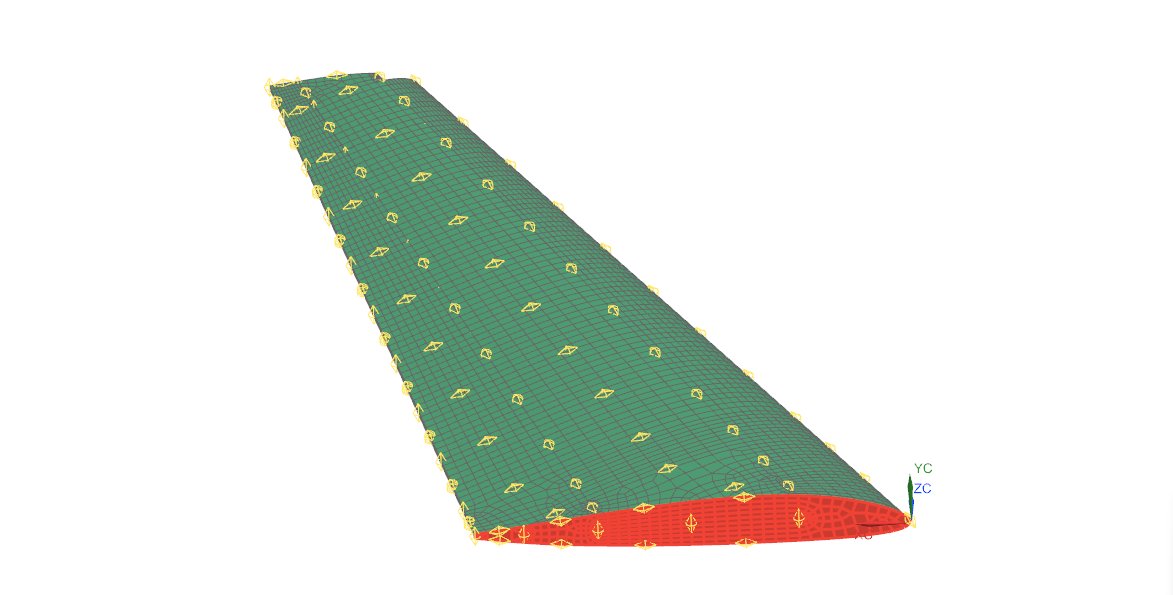
\includegraphics[width=0.75\textwidth]{figs/bc_nx.png}
    \caption{Condição de fronteira de encastramento aplicada à nervura de raiz (zona a vermelho) no NX Nastran.}
    \label{fig:bc_nx}
\end{figure}

\subsection{Configuração da Análise Modal}

A análise modal foi executada através da solução SOL 103 do NX Nastran, com o método de Lanczos como algoritmo de extração de valores próprios, conforme descrito na Secção \ref{sec:freq_naturais}. Os parâmetros de controlo são apresentados na Tabela \ref{tab:sol103}.

\begin{table}[H]
\centering
\caption{Parâmetros de controlo da análise modal SOL 103 
no NX Nastran.}
\label{tab:sol103}
\renewcommand{\arraystretch}{1.4}
\begin{tabularx}{\textwidth}{p{5cm} X}
\toprule
\textbf{Parâmetro} & \textbf{Valor} \\
\midrule
Solução                             & SOL 103 \\
Método de extração                  & Lanczos \\
Número de modos calculados          & 10 \\
Gama de frequências                 
    & $0$ -- \SI{10000}{\hertz} \\
Normalização dos vetores próprios   
    & Pela massa ($m_i = 1$) \\
Amortecimento estrutural            & Não considerado \\
\bottomrule
\end{tabularx}
\end{table}

A normalização pela massa garante que as massas modais generalizadas são unitárias ($m_i = 1$) e que as rigidezes modais generalizadas são numericamente iguais ao quadrado das frequências naturais ($k_i = \omega_i^2$), conforme a Equação \eqref{eq:massas_rigidezes_modais}, facilitando a comparação entre os modos das duas configurações \cite{Nastran2014, Craig2006}.

\chapter{Variável de Estudo: Orientação das Nervuras}
\label{chap:variavel}

\section{Definição da Variável de Desenho}

A variável de desenho estudada neste trabalho é a orientação das \textit{ribs} relativamente ao plano de simetria da aeronave. Conforme demonstrado na Secção \ref{sec:efeitos_geometricos}, a orientação das nervuras influencia diretamente a rigidez torsional efetiva da caixa alar e, consequentemente, as frequências naturais dos modos de torção \cite{Niu1988, Megson2012}.

Na prática industrial, a orientação das nervuras é uma decisão de projeto que envolve compromissos entre eficiência estrutural, facilidade de fabrico e integração com outros sistemas da aeronave. Em asas enflechadas, existem duas filosofias predominantes \cite{Raymer2018, Niu1988}:

\begin{itemize}
    \item \textbf{Nervuras perpendiculares ao bordo de ataque}: orientadas seguindo o enflechamento da asa,são estruturalmente mais eficientes em asas enflechadas,resistindo diretamente às cargas de corte transmitidaspelo revestimento \cite{Megson2012};

    \item \textbf{Nervuras paralelas ao plano de simetria}: orientadas perpendicularmente ao eixo longitudinal da fuselagem, simplificam a integração estrutural com a fuselagem e o fabrico, mas são menos eficientes estruturalmente em asas com elevado ângulo de enflechamento \cite{Niu1988}.
\end{itemize}

\section{Configuração A --- Nervuras a 25° com o Plano 
de Simetria}

Na Configuração A, representada na Figura \ref{fig:config_a}, as nervuras são orientadas de forma a fazer um ângulo de 25° com o plano de simetria da aeronave. Dado que este é coincidente com o ângulo de enflechamento, $\Lambda = \ang{25}$, estas tornam-se aproximadamente perpendiculares ao bordo de ataque. Esta é a configuração estruturalmente mais convencional para asas enflechadas e corresponde à solução adotada na aeronave real \cite{Niu1988, GarciaFernandez2025}.

A Configuração A possui um total de 13 nervuras, incluindo a nervura de raiz e a nervura de ponta, que são paralelas ao plano de simetria (0°) por razões de ligação estrutural. As 11 nervuras intermédias são inclinadas a 25° com o seguinte espaçamento:

\begin{itemize}
    \item \textbf{3 primeiras nervuras} (a partir da raiz): 
    espaçamento de \SI{317}{\milli\meter};
    \item \textbf{Restantes nervuras}: espaçamento de 
    \SI{436}{\milli\meter}.
\end{itemize}

\begin{table}[H]
\centering
\caption{Características geométricas da Configuração A.}
\label{tab:config_a}
\renewcommand{\arraystretch}{1.4}
\begin{tabularx}{\textwidth}{p{6cm} X}
\toprule
\textbf{Parâmetro} & \textbf{Valor} \\
\midrule
Número total de nervuras            & 13 \\
Ângulo das nervuras intermédias     
    & $\ang{25}$ com o plano de simetria \\
Ângulo das nervuras de raiz e ponta 
    & $ \ang{0}$ \\
Espaçamento --- 3 primeiras         
    & \SI{317}{\milli\meter} \\
Espaçamento --- restantes           
    & \SI{436}{\milli\meter} \\
\bottomrule
\end{tabularx}
\end{table}

É de notar que, na zona de interseção da nervura de ponta com o bordo de ataque, a inclinação de 25° das nervuras intermédias gerava uma geometria de difícil discretização, com problemas de densidade e continuidade da malha. Esta zona foi cortada de forma a garantir a qualidade da malha, sem comprometer a integridade estrutural do modelo \cite{Bathe2014, Cook2001}.

% FIGURA: Vista da Configuração A
\begin{figure}[H]
    \centering
    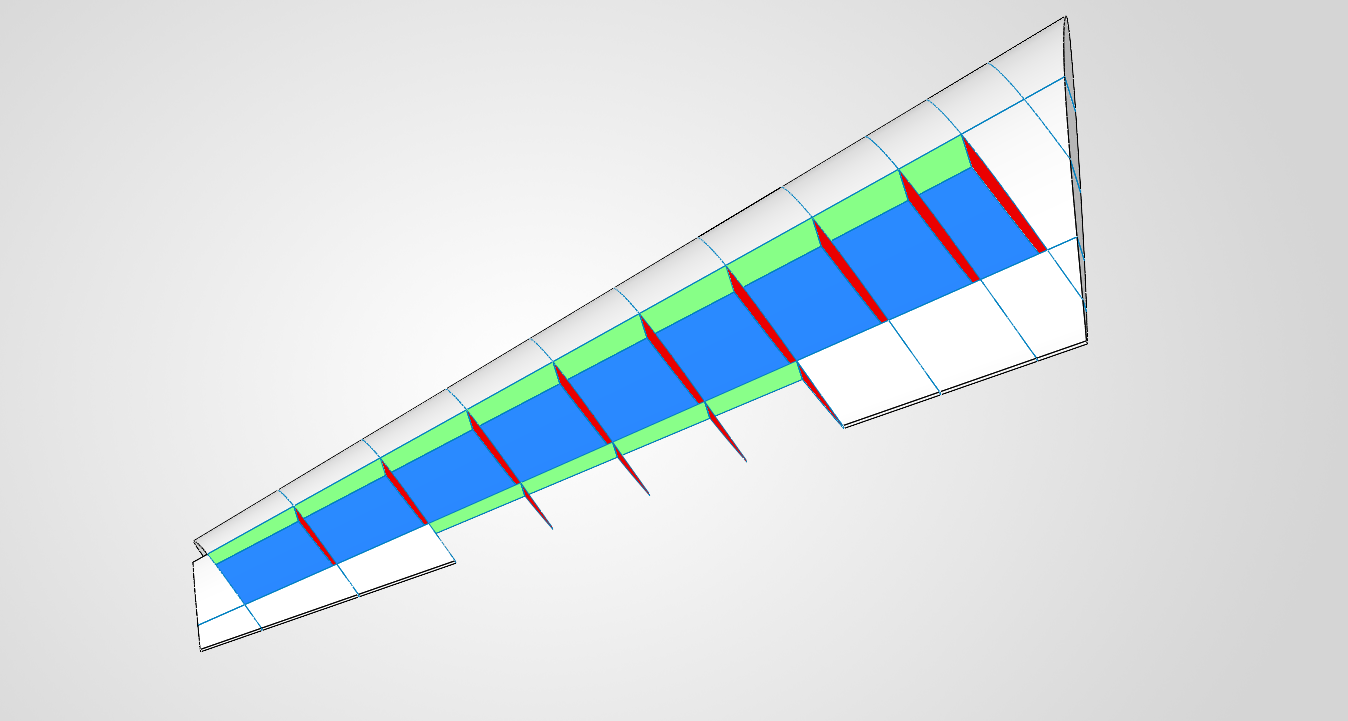
\includegraphics[width=0.85\textwidth]{figs/config_a.png}
    \caption{Vista da estrutura interna da Configuração A, com as nervuras orientadas a 25° relativamente ao plano de simetria da aeronave. O revestimento superior foi omitido para permitir a visualização da estrutura interna. O código de cores é análogo ao da Figura \ref{fig:asa_sw}.}
    \label{fig:config_a}
\end{figure}

\section{Configuração B --- Nervuras Paralelas ao Plano 
de Simetria}

Na Configuração B, representada na Figura \ref{fig:config_b}, as nervuras são orientadas a 0° com o plano de simetria da aeronave, ou seja, perpendiculares ao eixo longitudinal da fuselagem. Esta configuração possui um total de 10 nervuras, com espaçamento uniforme de \SI{443}{\milli\meter} entre todas as nervuras consecutivas.

\begin{table}[H]
\centering
\caption{Características geométricas da Configuração B.}
\label{tab:config_b}
\renewcommand{\arraystretch}{1.4}
\begin{tabularx}{\textwidth}{p{6cm} X}
\toprule
\textbf{Parâmetro} & \textbf{Valor} \\
\midrule
Número total de nervuras    & 10 \\
Ângulo das nervuras         
    & $ \ang{0}$ (paralelas ao plano de simetria) \\
Espaçamento entre nervuras  
    & \SI{443}{\milli\meter} (uniforme) \\
\bottomrule
\end{tabularx}
\end{table}

% FIGURA: Vista da Configuração B
\begin{figure}[H]
    \centering
    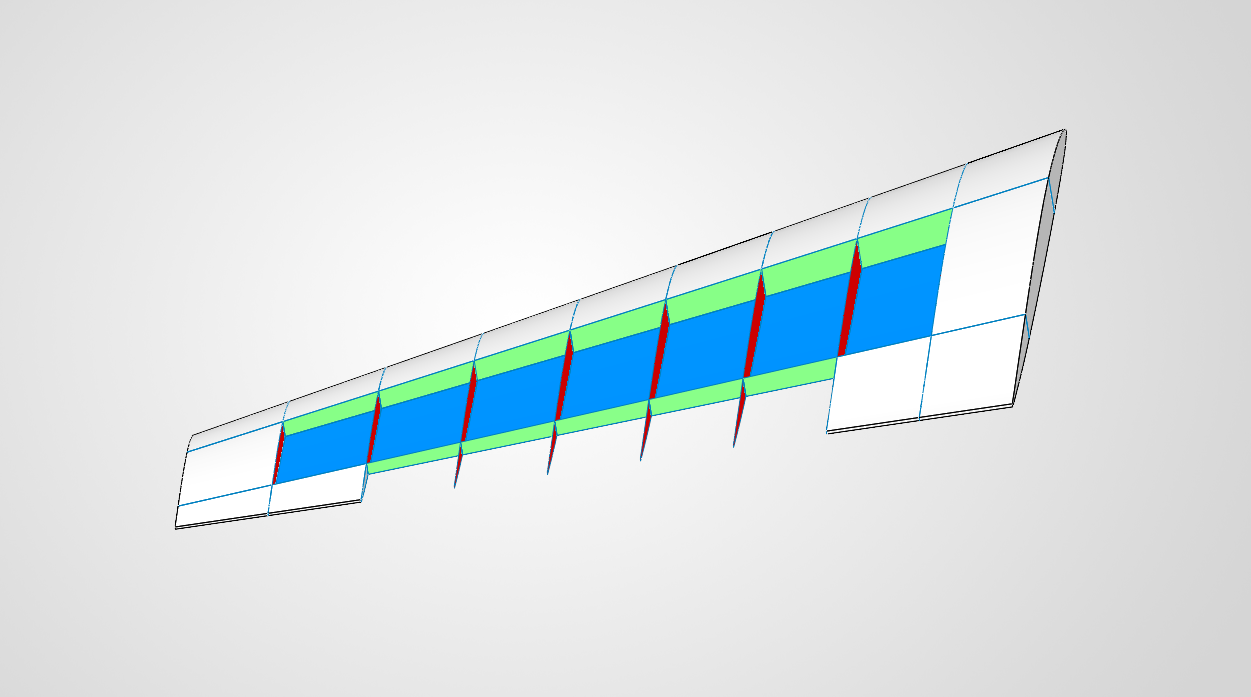
\includegraphics[width=0.85\textwidth]{figs/config_b.png}
    \caption{Vista da estrutura interna da Configuração B, com as nervuras orientadas a 0° relativamente ao plano de simetria da aeronave. O código de cores é análogo ao da Figura \ref{fig:asa_sw}.}
    \label{fig:config_b}
\end{figure}

\section{Comparação entre Configurações}

A Tabela \ref{tab:comparacao_configs} apresenta uma comparação direta entre as duas configurações, evidenciando as principais diferenças geométricas e estruturais.

\begin{table}[H]
\centering
\caption{Comparação entre a Configuração A e a Configuração B.}
\label{tab:comparacao_configs}
\renewcommand{\arraystretch}{1.4}
\begin{tabularx}{\textwidth}{l >{\raggedright\arraybackslash}X >{\raggedright\arraybackslash}X}
\toprule
\textbf{Parâmetro} & \textbf{Configuração A} & \textbf{Configuração B} \\
\midrule
Ângulo das nervuras & $\ang{25}$ c/ plano de simetria & $\ang{0}$ \\
Número de nervuras & 13 & 10 \\
Espaçamento & \SI{317}{\milli\meter} (3 primeiras) e \SI{436}{\milli\meter} (restantes) & \SI{443}{\milli\meter} (uniforme) \\
Relação c/ bordo de ataque & Aproximadamente perpendiculares & Oblíquas \\
Massa total das nervuras & Superior (mais nervuras) & Inferior \\
Rigidez torsional esperada & Superior & Inferior \\
Representatividade real & Configuração real do AN-124 & Configuração alternativa \\
\bottomrule
\end{tabularx}
\end{table}

Do ponto de vista estrutural, as nervuras perpendiculares ao bordo de ataque (Configuração A) são mais eficientes na resistência às tensões de corte induzidas pela torção, uma vez que estão alinhadas com as trajetórias de fluxo de corte naturais da caixa alar enflechada, garantindo uma transmissão de cargas mais direta entre o revestimento e as longarinas \cite{Niu1988, Megson2012}. As nervuras paralelas ao eixo da fuselagem (Configuração B) introduzem componentes de força fora do plano da nervura, reduzindo a eficiência estrutural mas simplificando o processo de fabrico \cite{Raymer2018}.

É importante notar que as duas configurações diferem não apenas na orientação das nervuras, mas também no número total (13 vs 10) e no espaçamento entre elas. Estas diferenças são consequência direta da variável de desenho estudada: ao alterar a orientação das nervuras mantendo a coerência geométrica da estrutura, o número e espaçamento necessariamente se alteram para cobrir adequadamente a envergadura da asa. A influência conjunta destas diferenças sobre as frequências naturais e formas modais será analisada no Capítulo \ref{chap:resultados} \cite{Wright2015, Dowell2004}.

\chapter{Resultados e Discussão}
\label{chap:resultados}

\section{Frequências Naturais --- Configuração A}

Os resultados da análise modal da Configuração A, obtidos através da solução SOL 103 do NX Nastran com o método de Lanczos, são apresentados na Tabela \ref{tab:freqs_a}. Foram extraídos os primeiros 10 modos de vibração, correspondentes às 10 menores frequências naturais da estrutura.


\begin{table}[H]
\centering
\caption{Frequências naturais dos 10 primeiros modos de vibração da Configuração A.}
\label{tab:freqs_a}
\renewcommand{\arraystretch}{1.4}
\begin{tabular*}{\textwidth}{@{\extracolsep{\fill}} l l l l @{}}
\toprule
\textbf{Modo} & \textbf{Freq. [\si{\hertz}]} & \textbf{Tipo} & \textbf{Descrição} \\
\midrule
1  & \texttt{14.83} & Flexão & 1º modo de flexão (1B) \\
2  & \texttt{57.39} & Flexão & 2º modo de flexão (2B) \\
3  & \texttt{84.61} & Flexão & 3º modo de flexão (3B) \\
4  & \texttt{89.55} & Torção & 1º modo de torção (1T) \\
5  & \texttt{95.55} & Flexão & 4º modo de flexão (4B) \\
6  & \texttt{99.82} & Torção & 2º modo de torção (2T) \\
7  & \texttt{100.94} & Flexão & 5º modo de flexão (5B) \\
8  & \texttt{105.87} & Flexão & 6º modo de flexão (6B) \\
9  & \texttt{109.62} & Torção & 3º modo de torção (3T) \\
10 & \texttt{113.47} & Flexão & 7º modo de flexão (7B) \\
\bottomrule
\end{tabular*}
\end{table}

\section{Frequências Naturais --- Configuração B}

Os resultados da análise modal da Configuração B são apresentados na Tabela \ref{tab:freqs_b}, obtidos nas mesmas condições de análise da Configuração A.

\begin{table}[H]
\centering
\caption{Frequências naturais dos 10 primeiros modos de vibração da Configuração B.}
\label{tab:freqs_b}
\renewcommand{\arraystretch}{1.4}
\begin{tabular*}{\textwidth}{@{\extracolsep{\fill}} l l l l @{}}
\toprule
\textbf{Modo} & \textbf{Freq. [\si{\hertz}]} & \textbf{Tipo} & \textbf{Descrição} \\
\midrule
1  & \texttt{14.76}  & Flexão & 1º modo de flexão (1B) \\
2  & \texttt{56.82}  & Flexão & 2º modo de flexão (2B) \\
3  & \texttt{84.36}  & Flexão & 3º modo de flexão (3B) \\
4  & \texttt{89.45}  & Torção & 1º modo de torção (1T) \\
5  & \texttt{90.43}  & Flexão & 4º modo de flexão (4B) \\
6  & \texttt{95.64}  & Torção & 2º modo de torção (2T) \\
7  & \texttt{96.30}  & Flexão & 5º modo de flexão (5B) \\
8  & \texttt{96.58}  & Torção & 3º modo de torção (3T) \\
9  & \texttt{101.37} & Flexão & 6º modo de flexão (6B) \\
10 & \texttt{102.61} & Torção & 4º modo de torção (4T) \\
\bottomrule
\end{tabular*}
\end{table}

\section{Formas Modais --- Configuração A}

As formas modais dos três primeiros modos de flexão e do primeiro modo de torção da Configuração A são apresentadas nas Figuras \ref{fig:modo1a} a \ref{fig:modo_torcao_a}. As formas modais foram obtidas diretamente do NX Nastran e visualizadas através do mapa de deslocamentos nodais normalizado pela massa, conforme descrito na Secção \ref{sec:analise_modal_aero}.


% FIGURA: 1º modo de flexão --- Configuração A
\begin{figure}[H]
    \centering
    % Primeira Subfigura
    \subfloat[Vista 1.\label{fig:modo1a_v1}]{
        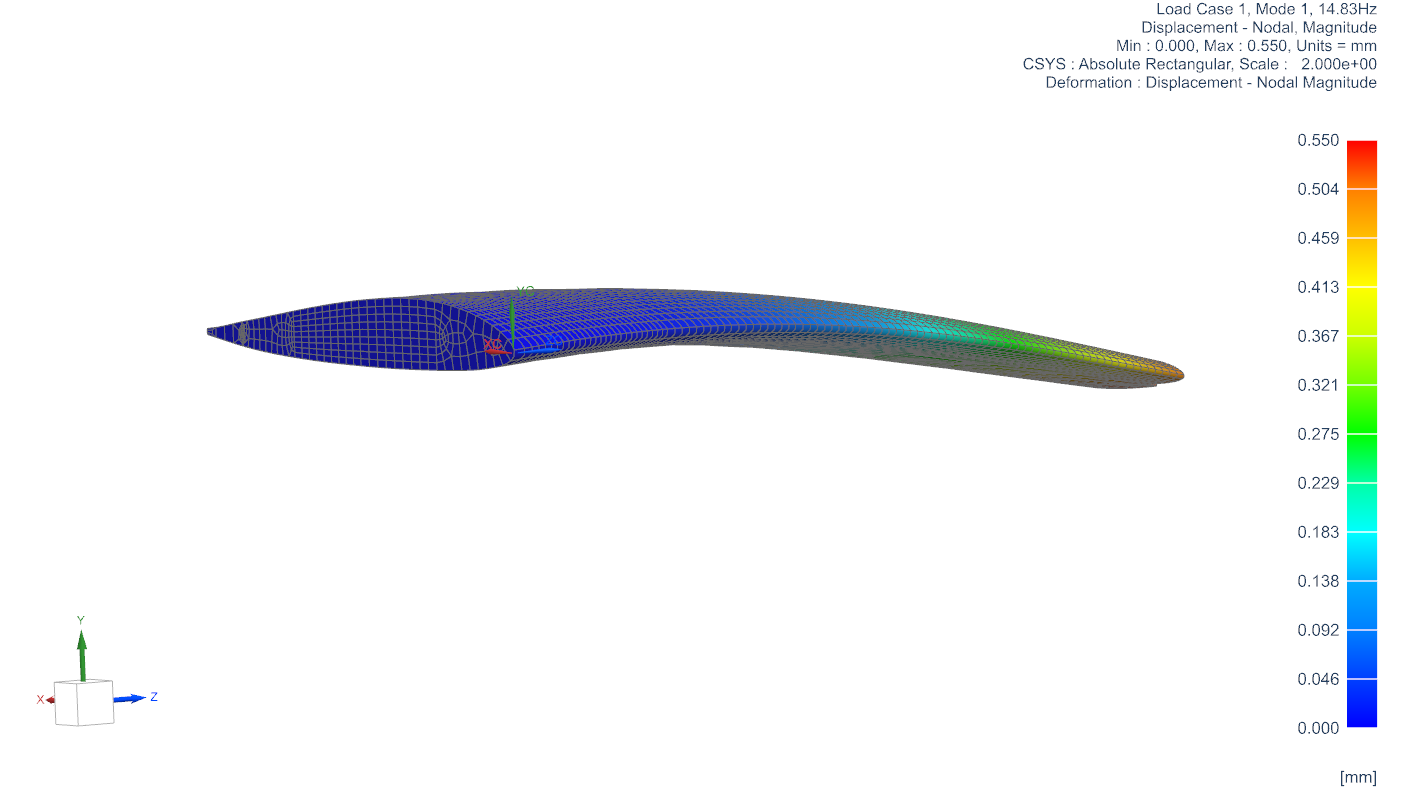
\includegraphics[width=0.45\textwidth]{figs/modo1_confA_vista1.png}
    }
    \hfill % Espaçamento horizontal
    % Segunda Subfigura
    \subfloat[Vista 2.\label{fig:modo1a_v2}]{
        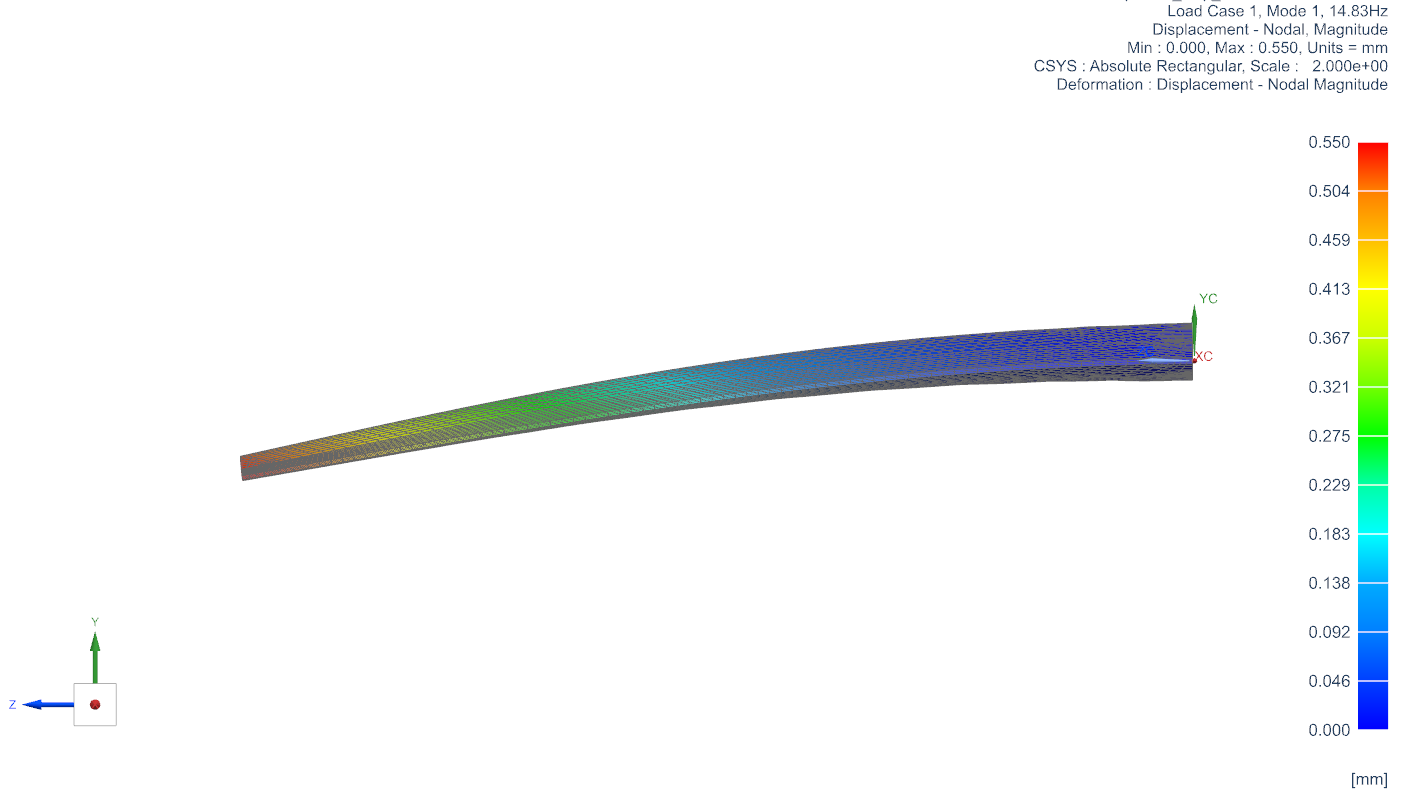
\includegraphics[width=0.45\textwidth]{figs/modo1_confA_vista2.png}
    }

    \caption{Primeiro modo de flexão (1B) da Configuração A. A deformação é dominantemente na direção vertical, com amplitude máxima na ponta da asa e nó de vibração na raiz encastrada. Frequência natural: \texttt{14.83}~Hz.}
    \label{fig:modo1a}
\end{figure}

O primeiro modo de flexão (1B) é o modo de menor frequência da estrutura e caracteriza-se por uma deformação predominantemente fora do plano (\textit{out-of-plane bending}), com a amplitude máxima de deslocamento concentrada na ponta da asa e um único nó de vibração na secção de raiz encastrada \cite{Bisplinghoff1996}. Devido ao enflechamento de $\qty{25}{\degree}$ e ao acoplamento flexão-torção descrito na Secção \ref{sec:sweep}, este modo apresenta uma componente de torção não nula, visível na rotação diferencial das secções ao longo da envergadura \cite{Wright2015}.


% FIGURA: 2º modo de flexão --- Configuração A
\begin{figure}[H]
    \centering
    % Primeira Subfigura
    \subfloat[Vista 1.\label{fig:modo2a_v1}]{
        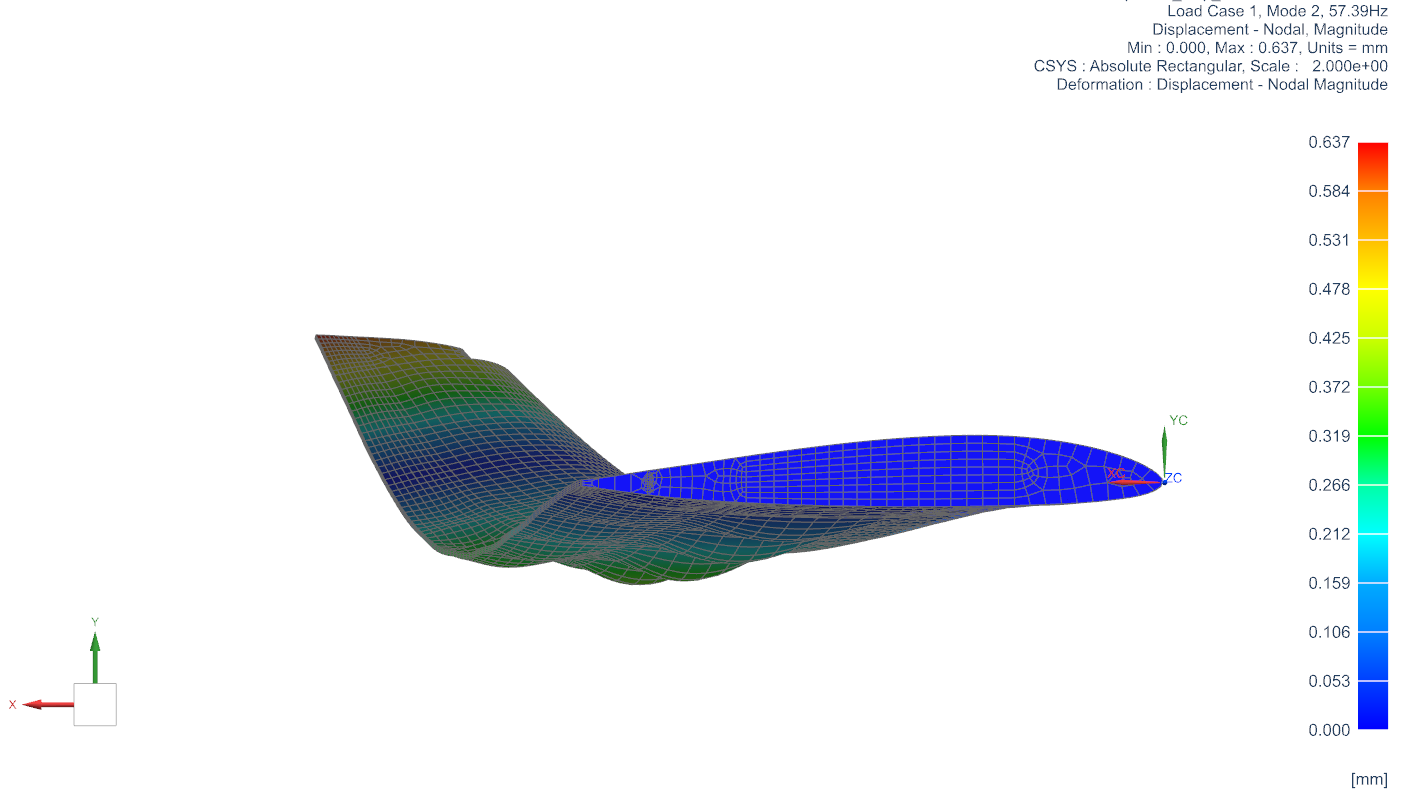
\includegraphics[width=0.45\textwidth]{figs/modo2_confA_vista1.png}
    }
    \hfill % Espaçamento horizontal
    % Segunda Subfigura
    \subfloat[Vista 2.\label{fig:modo2a_v2}]{
        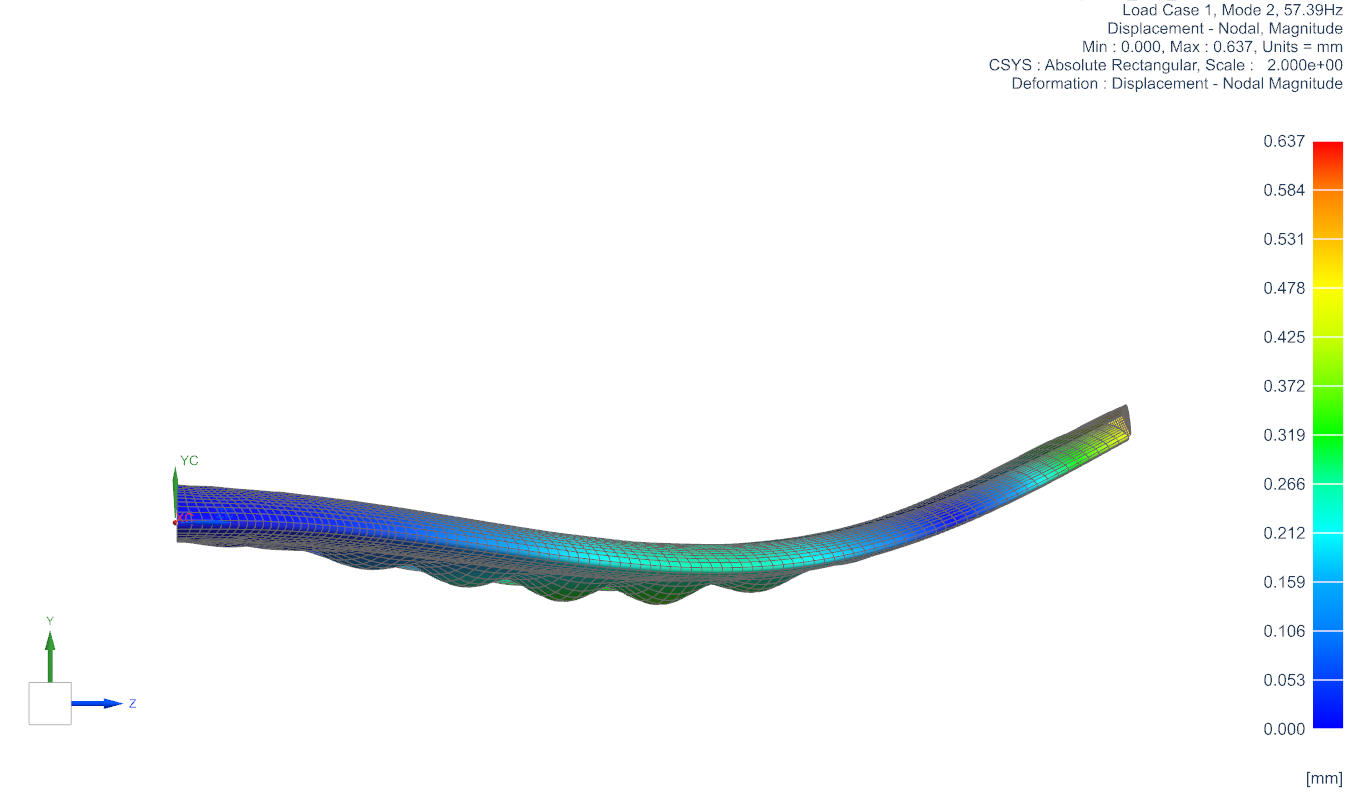
\includegraphics[width=0.45\textwidth]{figs/modo2_confA_vista2.png}
    }
    \caption{Segundo modo de flexão (2B) da Configuração A, 
    com um nó de vibração intermédio ao longo da envergadura. 
    Frequência natural: \texttt{57.39}~\si{\hertz}.}
    \label{fig:modo2a}
\end{figure}

O segundo modo de flexão (2B) caracteriza-se pela presença de um nó de vibração livre ao longo da envergadura, para além do nó imposto pela condição de encastramento na raiz, conferindo à deformada modal uma configuração em S \cite{Rao2011}. A frequência deste modo é tipicamente superior à do modo 1B por um fator próximo de $(4.694/1.875)^2 \approx 6.27$, conforme previsto pela teoria da viga em consola, Equação \eqref{eq:freq_viga} \cite{Rao2011}.


% FIGURA: 3º modo de flexão --- Configuração A
\begin{figure}[H]
    \centering
    % Primeira Subfigura
    \subfloat[Vista 1.\label{fig:modo3a_v1}]{
        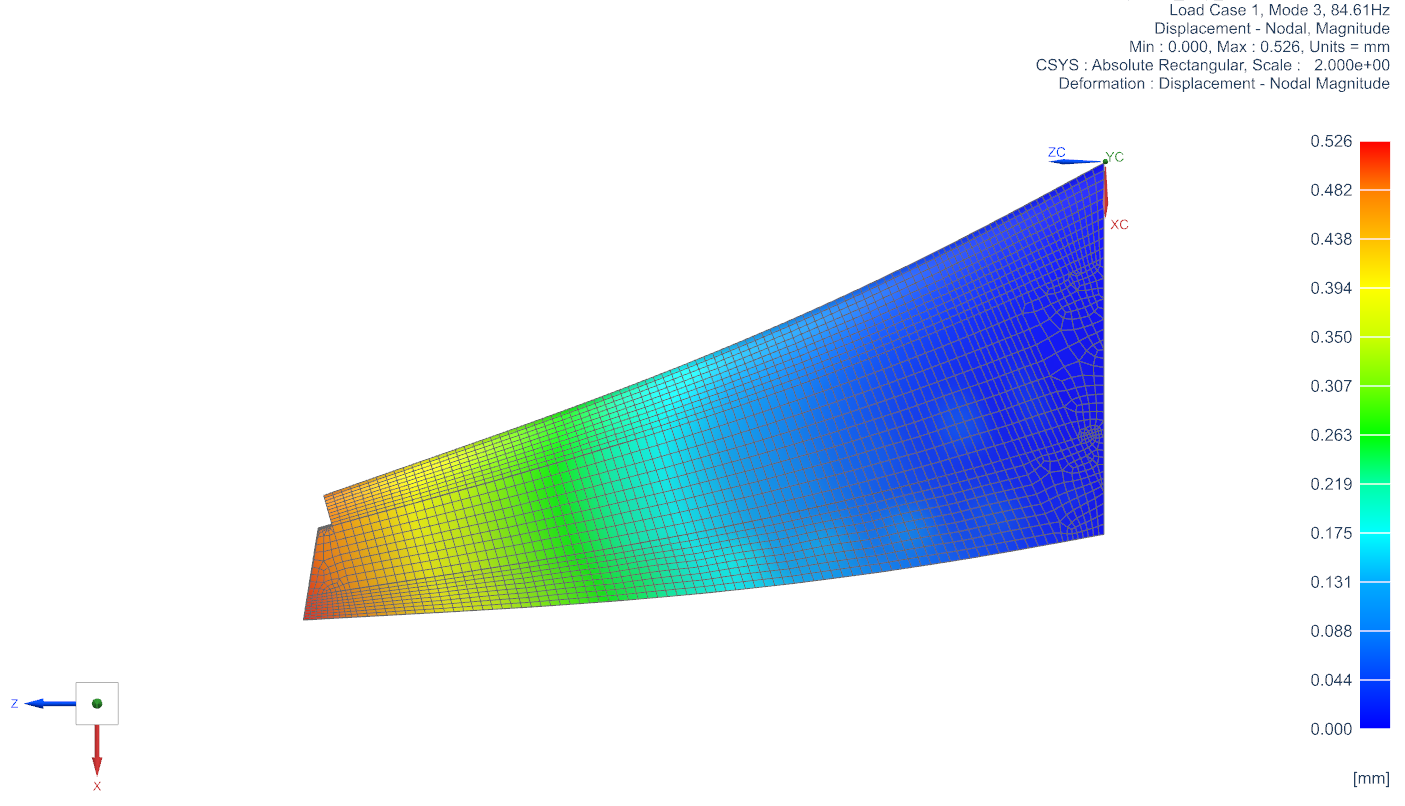
\includegraphics[width=0.45\textwidth]{figs/modo3_confA_vista1.png}
    }
    \hfill % Espaçamento horizontal
    % Segunda Subfigura
    \subfloat[Vista 2.\label{fig:modo3a_v2}]{
        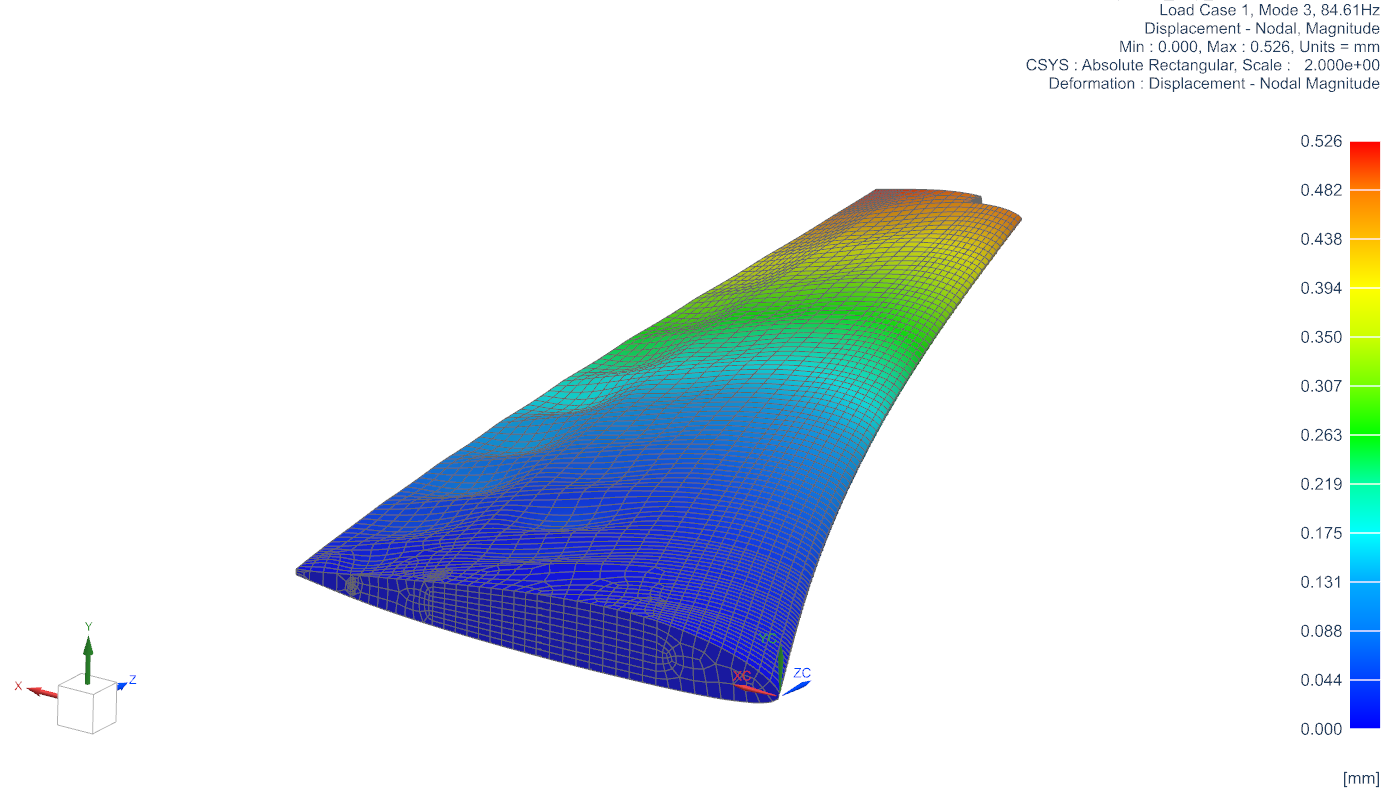
\includegraphics[width=0.45\textwidth]{figs/modo3_confA_vista2.png}
    }
    \caption{Terceiro modo de flexão (3B) da Configuração A, 
    com dois nós de vibração intermédios ao longo da 
    envergadura. Frequência natural: 
    \texttt{84.61}~\si{\hertz}.}
    \label{fig:modo3a}
\end{figure}


% FIGURA: 1º modo de torção --- Configuração A
\begin{figure}[H]
    \centering
    % Primeira Subfigura
    \subfloat[Vista 1.\label{fig:modo4a_v1}]{
        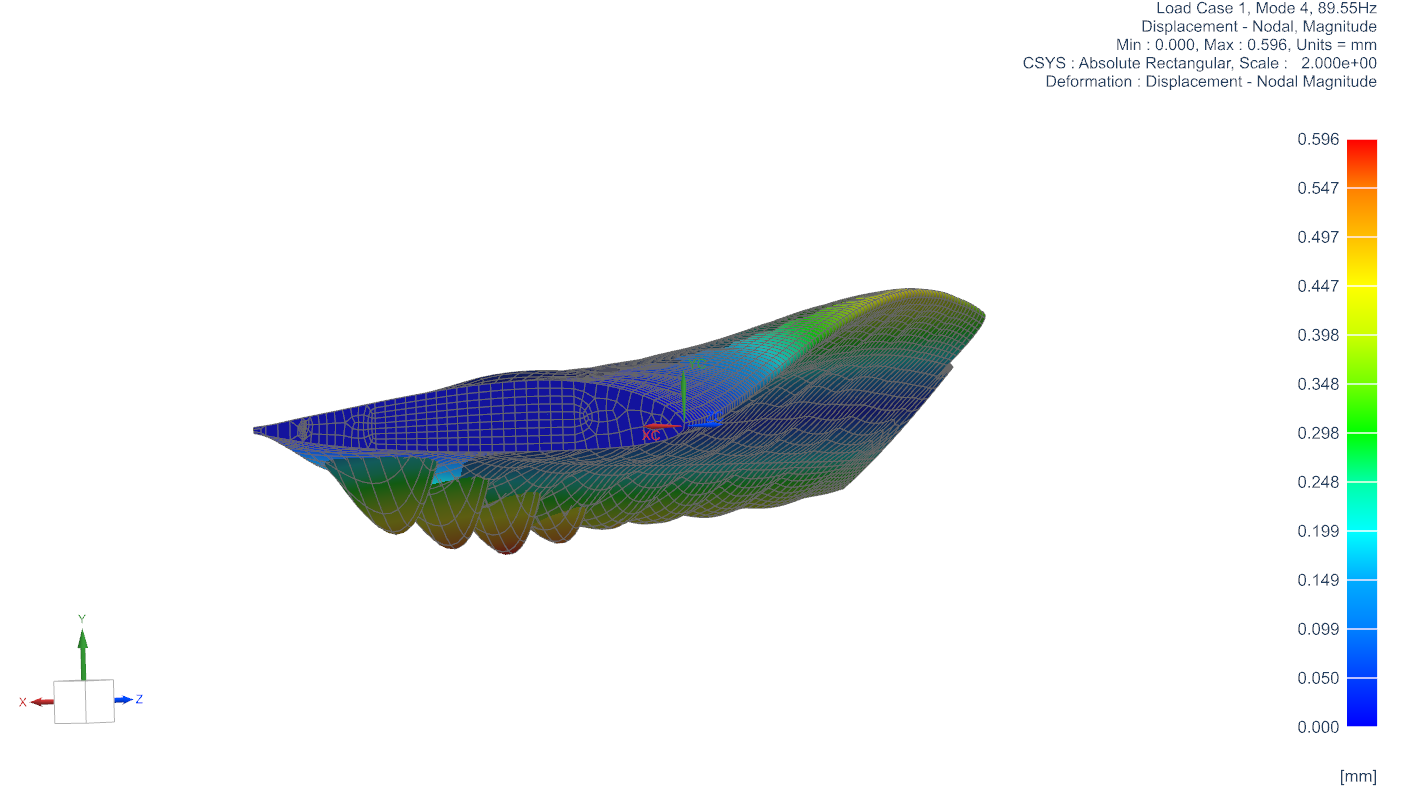
\includegraphics[width=0.45\textwidth]{figs/modo4_confA_vista1.png}
    }
    \hfill % Espaçamento horizontal
    % Segunda Subfigura
    \subfloat[Vista 2.\label{fig:modo4a_v2}]{
        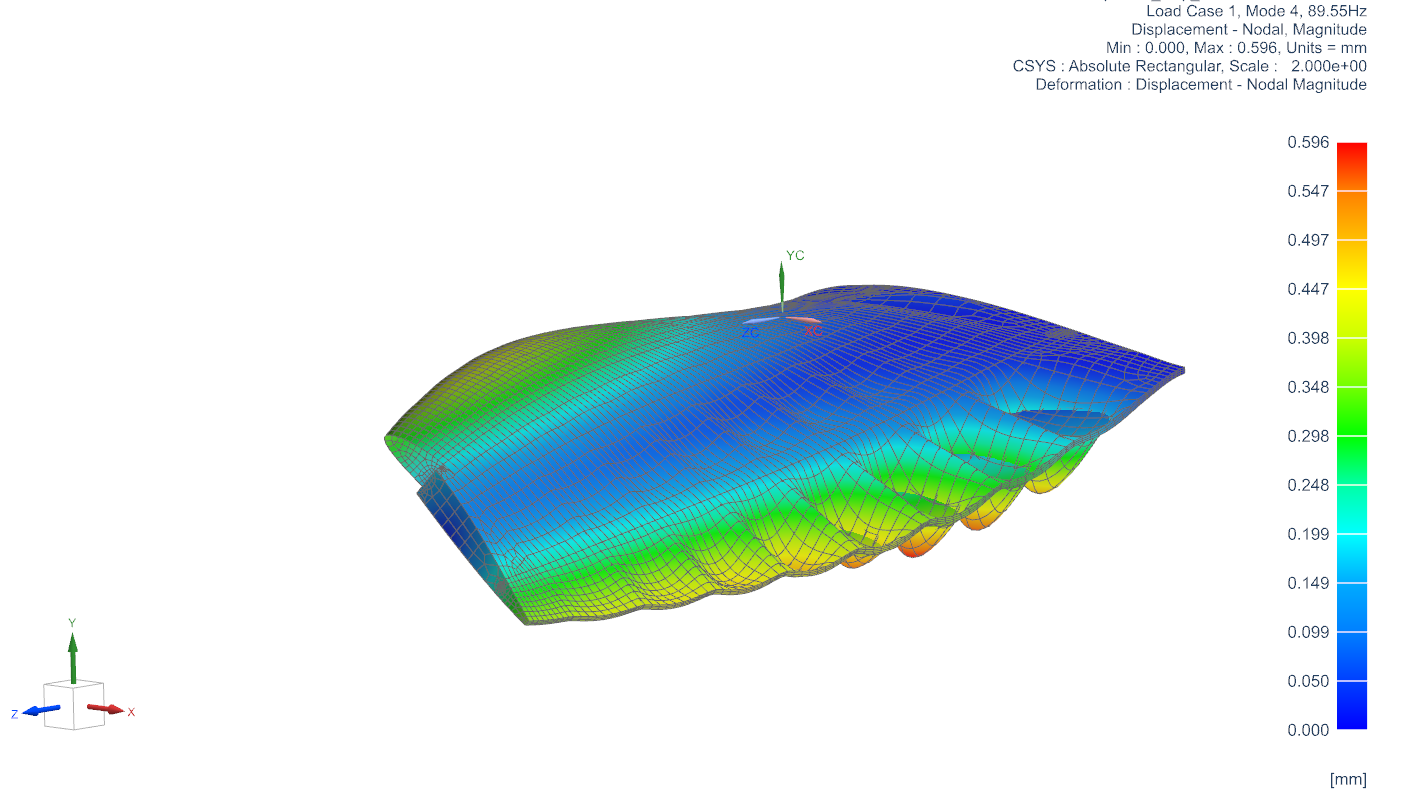
\includegraphics[width=0.45\textwidth]{figs/modo4_confA_vista2.png}
    }
    \caption{Primeiro modo de torção (1T) da Configuração A. A deformação é dominantemente torsional, com rotação crescente ao longo da envergadura e amplitude máxima na ponta da asa. Frequência natural: 
    \texttt{89.55}~\si{\hertz}.}
    \label{fig:modo_torcao_a}
\end{figure}

O primeiro modo de torção (1T) caracteriza-se por uma rotação progressiva das secções da asa ao longo da envergadura, com amplitude nula na raiz (condição de encastramento) e máxima na ponta. A separação entre as frequências dos modos 1T e 1B, designada por \textit{flutter margin} no domínio modal, constitui um parâmetro fundamental para avaliar a propensão da estrutura ao acoplamento aeroelástico dinâmico \cite{Fung1993, Dowell2004}. Quanto menor esta separação, maior a probabilidade de \textit{flutter} a velocidades de voo mais baixas.

\section{Formas Modais --- Configuração B}

As formas modais dos três primeiros modos de flexão e do primeiro modo de torção da Configuração B são apresentadas nas Figuras \ref{fig:modo1b} a \ref{fig:modo_torcao_b}.

% FIGURA: 1º modo de flexão --- Configuração B
\begin{figure}[H]
    \centering
    % Primeira Subfigura
    \subfloat[Vista 1.\label{fig:modo1b_v1}]{
        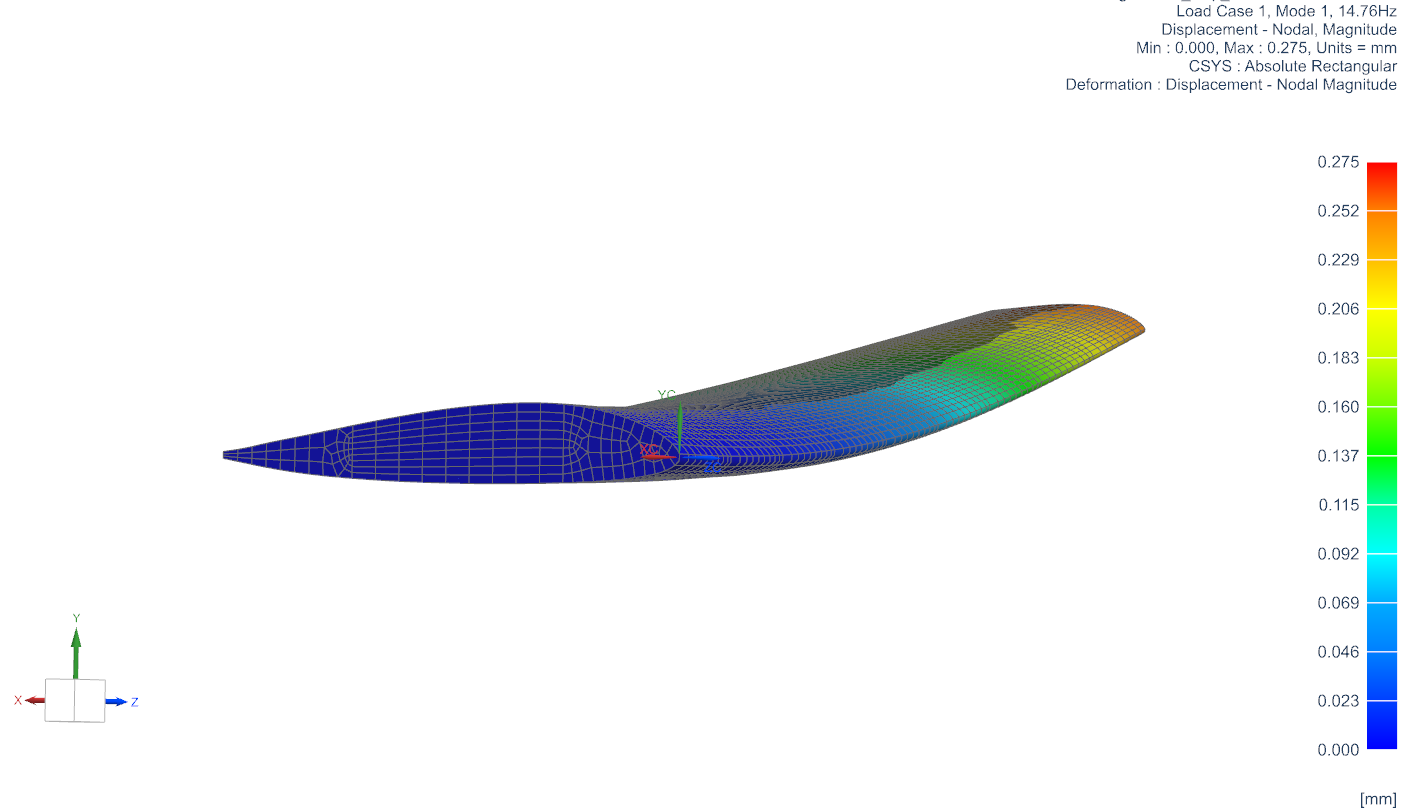
\includegraphics[width=0.45\textwidth]{figs/modo1_confB_vista1.png}
    }
    \hfill % Espaçamento horizontal
    % Segunda Subfigura
    \subfloat[Vista 2.\label{fig:modo1b_v2}]{
        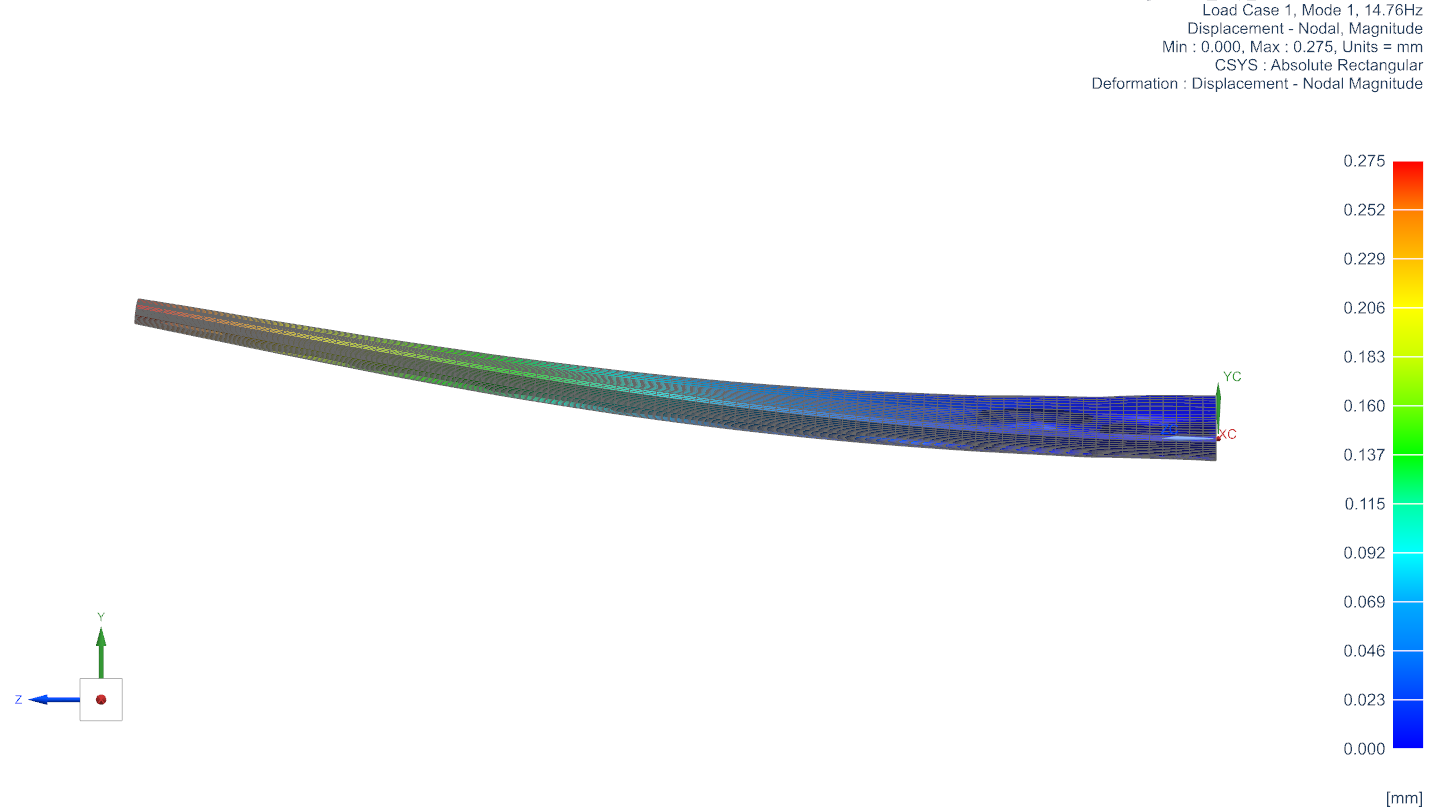
\includegraphics[width=0.45\textwidth]{figs/modo1_confB_vista2.png}
    }
    \caption{Primeiro modo de flexão (1B) da Configuração B. 
    Frequência natural: \texttt{14.76}~\si{\hertz}.}
    \label{fig:modo1b}
\end{figure}

% FIGURA: 2º modo de flexão --- Configuração B
\begin{figure}[H]
    \centering
    % Primeira Subfigura
    \subfloat[Vista 1.\label{fig:modo2b_v1}]{
        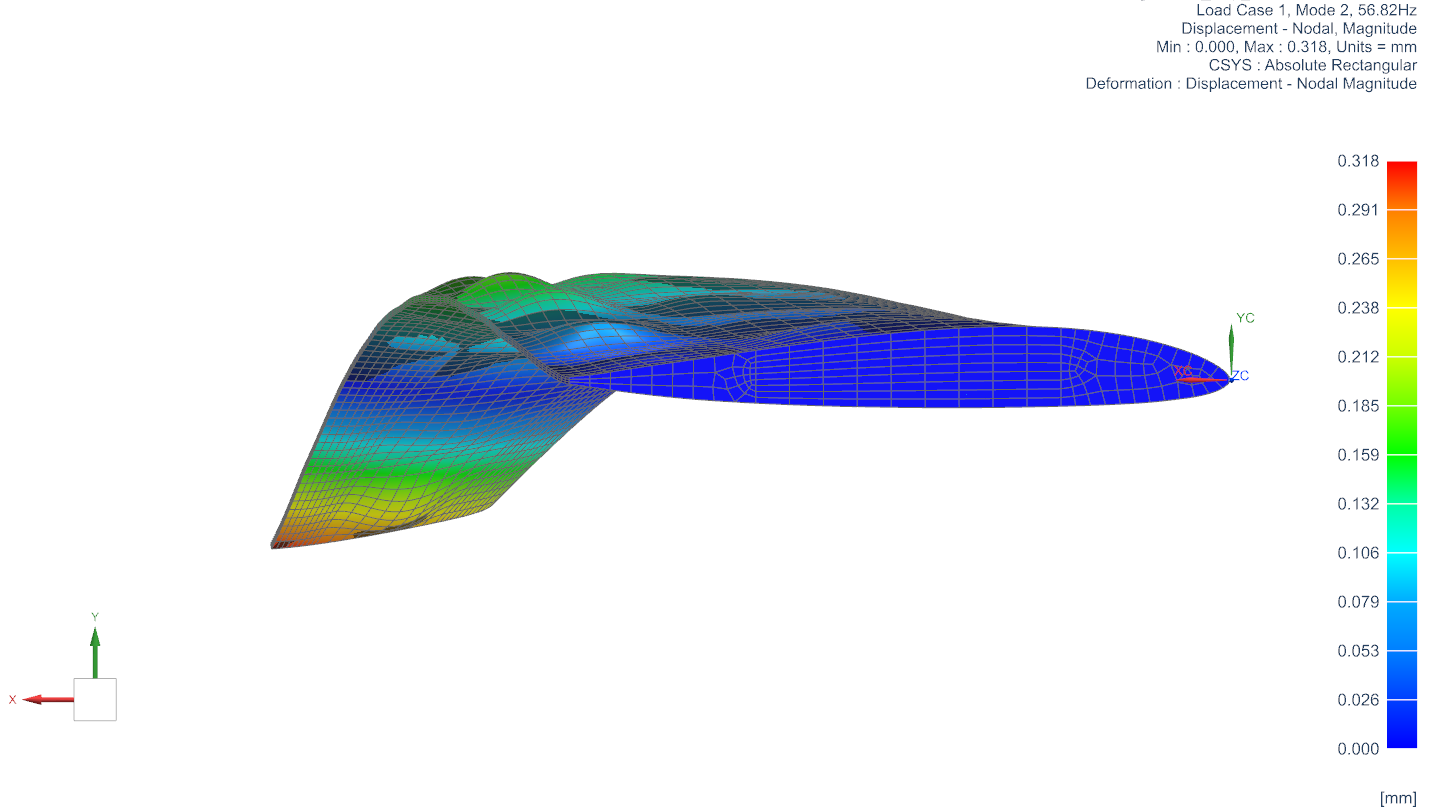
\includegraphics[width=0.45\textwidth]{figs/modo2_confB_vista1.png}
    }
    \hfill % Espaçamento horizontal
    % Segunda Subfigura
    \subfloat[Vista 2.\label{fig:modo2b_v2}]{
        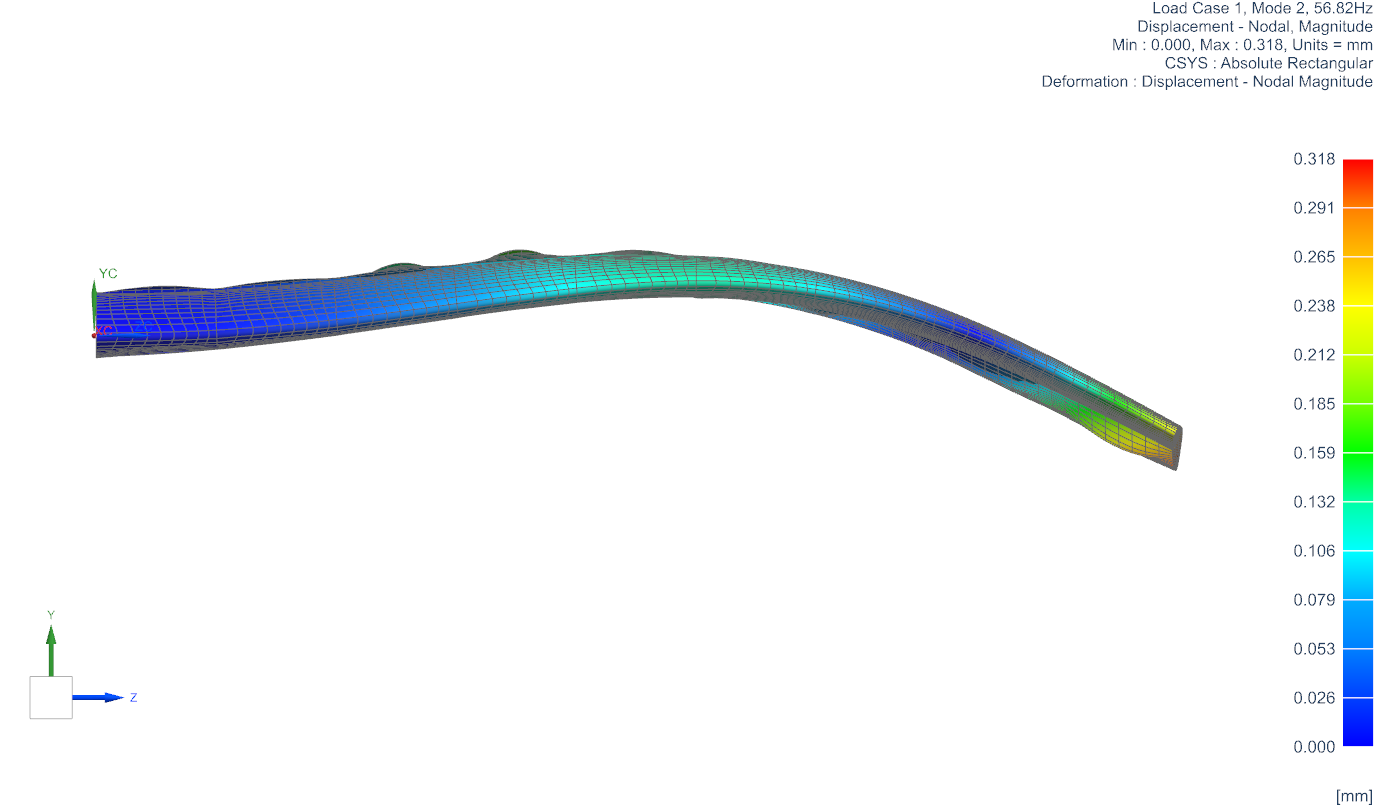
\includegraphics[width=0.45\textwidth]{figs/modo2_confB_vista2.png}
    }
    \caption{Segundo modo de flexão (2B) da Configuração B. 
    Frequência natural: \texttt{56.82}~\si{\hertz}.}
    \label{fig:modo2b}
\end{figure}


% FIGURA: 3º modo de flexão --- Configuração B
\begin{figure}[H]
    \centering
    % Primeira Subfigura
    \subfloat[Vista 1.\label{fig:modo3b_v1}]{
        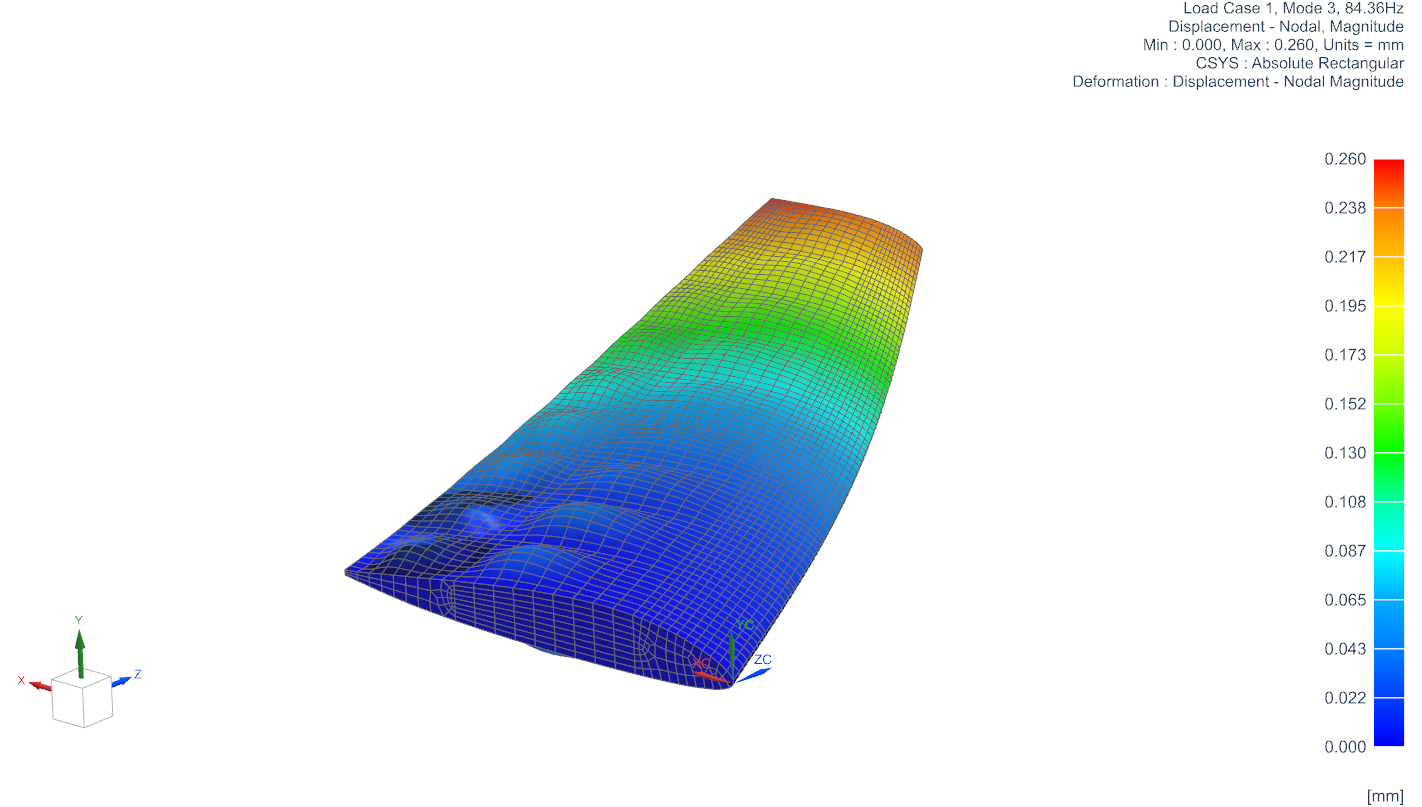
\includegraphics[width=0.45\textwidth]{figs/modo3_confB_vista1.png}
    }
    \hfill % Espaçamento horizontal
    % Segunda Subfigura
    \subfloat[Vista 2.\label{fig:modo3b_v2}]{
        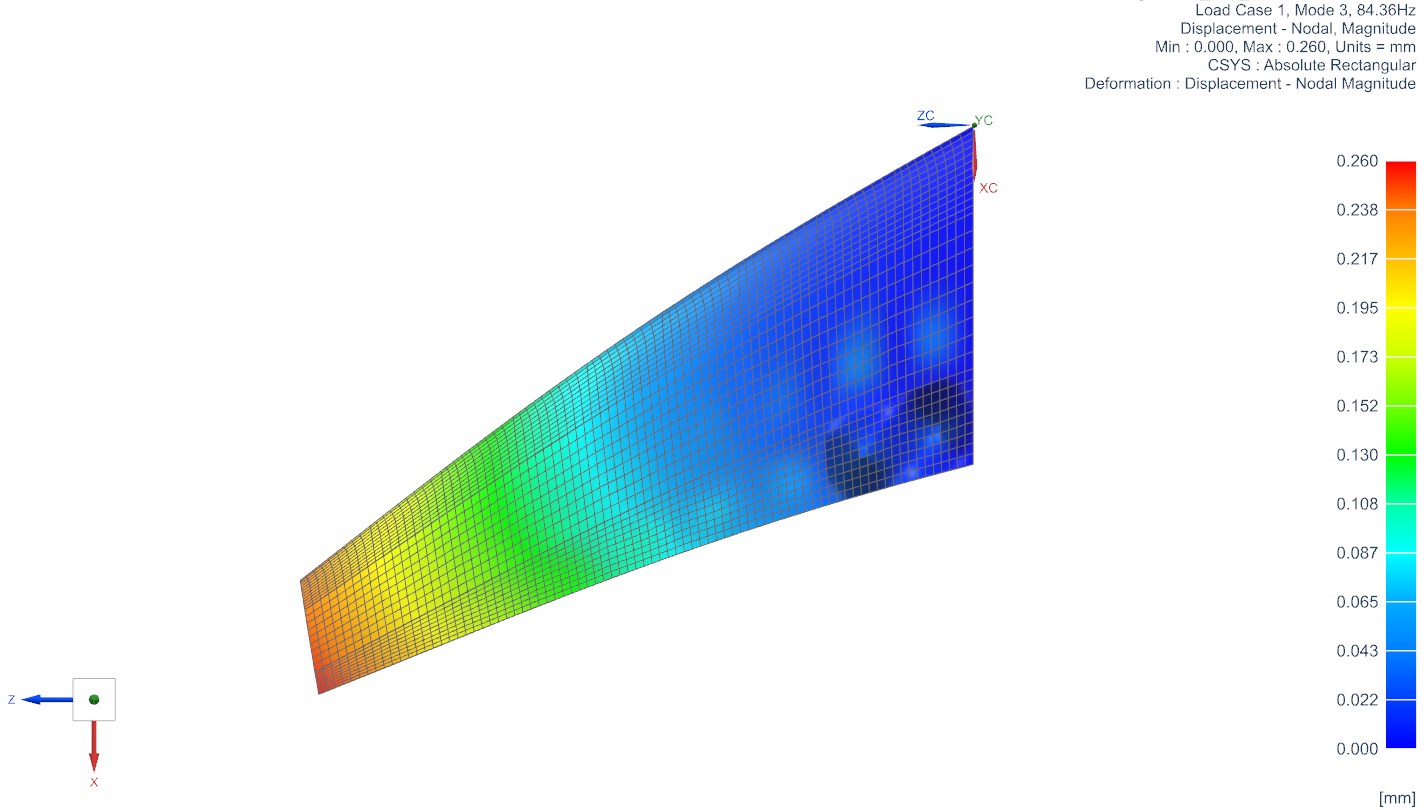
\includegraphics[width=0.45\textwidth]{figs/modo3_confB_vista2.png}
    }
    \caption{Terceiro modo de flexão (3B) da Configuração B. 
    Frequência natural: \texttt{84.36}~\si{\hertz}.}
    \label{fig:modo3b}
\end{figure}


% FIGURA: 1º modo de torção --- Configuração B
\begin{figure}[H]
    \centering
    % Primeira Subfigura
    \subfloat[Vista 1.\label{fig:modo4b_v1}]{
        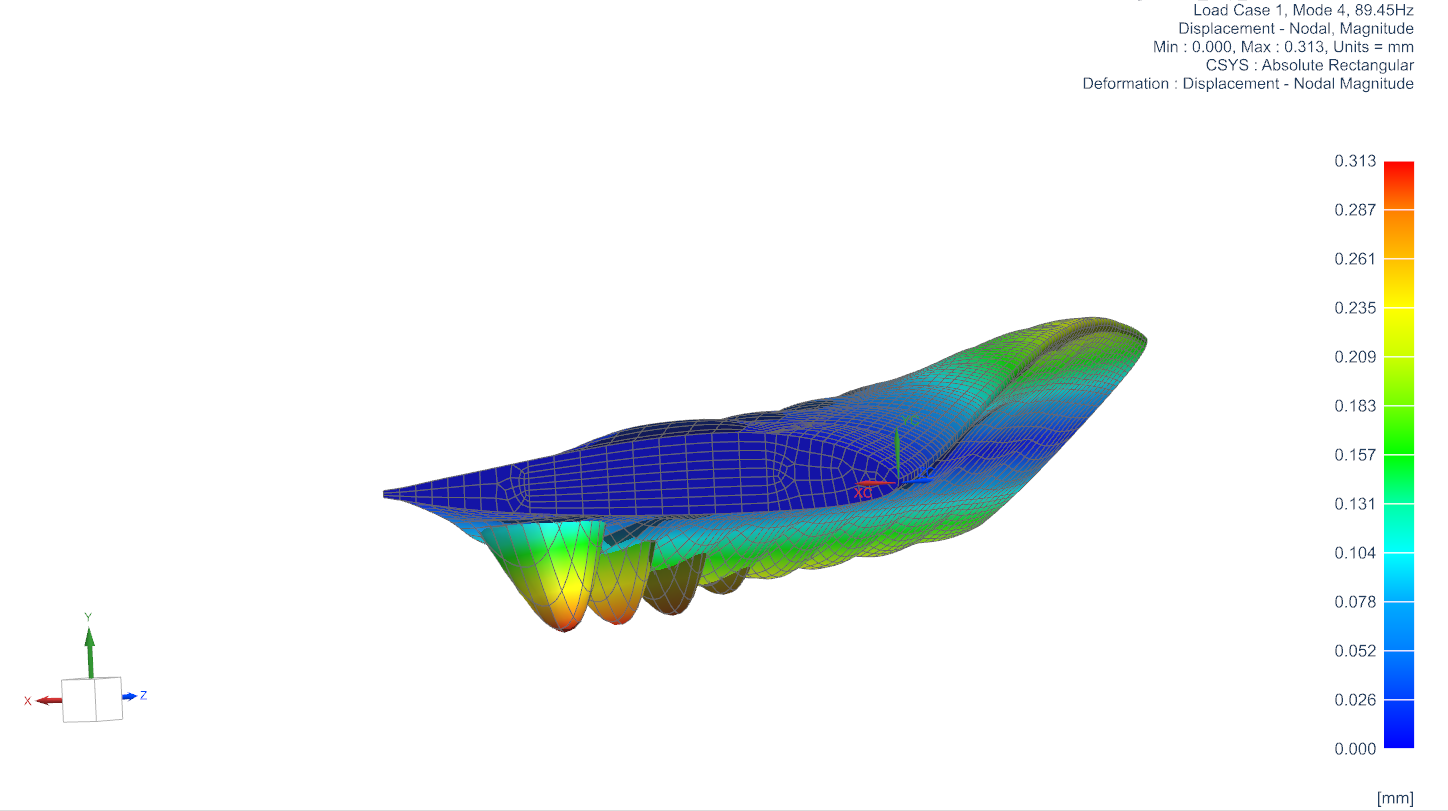
\includegraphics[width=0.45\textwidth]{figs/modo4_confB_vista1.png}
    }
    \hfill % Espaçamento horizontal
    % Segunda Subfigura
    \subfloat[Vista 2.\label{fig:modo4b_v2}]{
        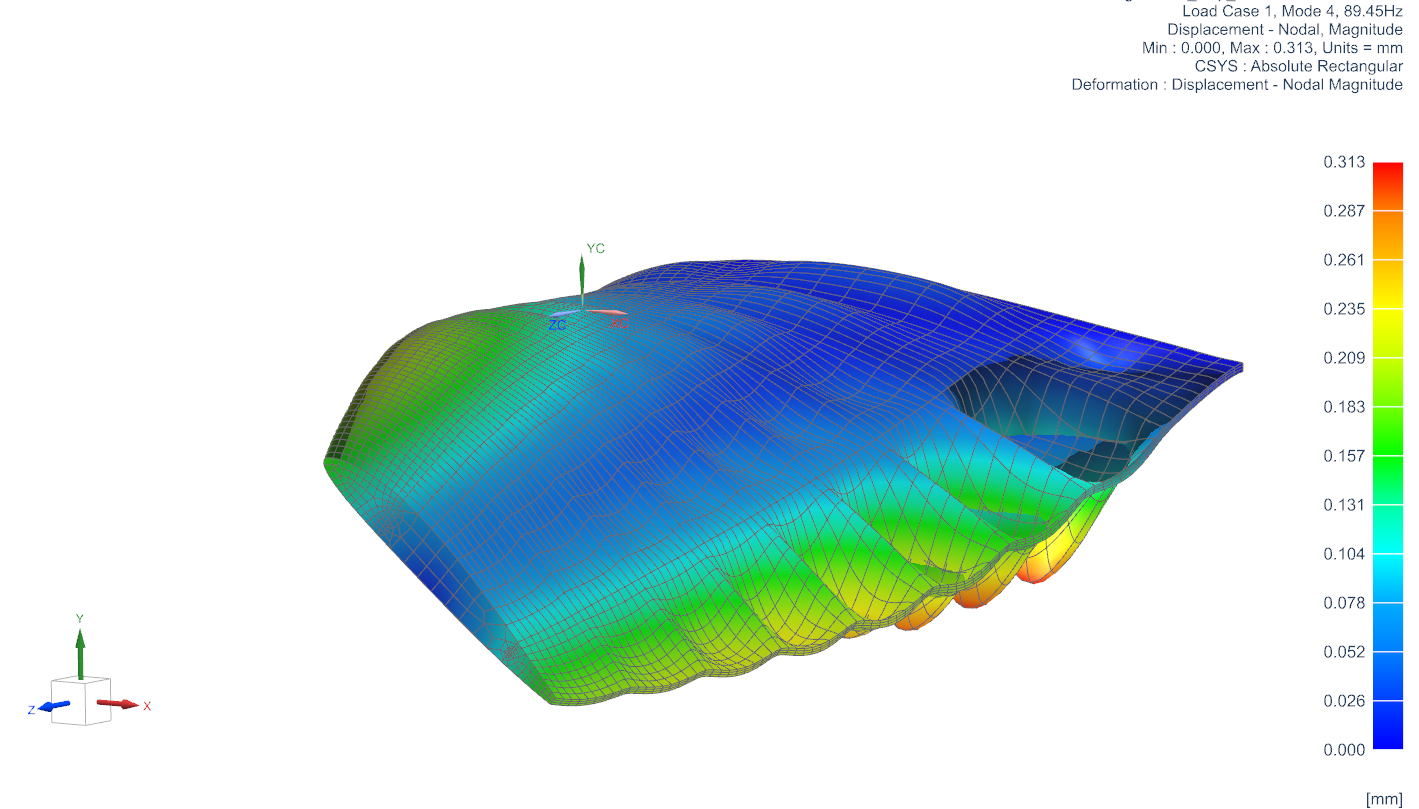
\includegraphics[width=0.45\textwidth]{figs/modo4_confB_vista2.png}
    }
    \caption{Primeiro modo de torção (1T) da Configuração B. 
    Frequência natural: \texttt{89.45}~\si{\hertz}.}
    \label{fig:modo_torcao_b}
\end{figure}

\section{Comparação entre Configurações}

\subsection{Comparação das Frequências Naturais}

A Tabela \ref{tab:comparacao_freqs} apresenta a comparação direta entre as frequências naturais dos modos de interesse nas duas configurações, bem como a variação relativa introduzida pela alteração da orientação das nervuras.

\begin{table}[H]
\centering
\caption{Comparação das frequências naturais entre as duas configurações para os modos de interesse.}
\label{tab:comparacao_freqs}
\renewcommand{\arraystretch}{1.4}
\begin{tabularx}{\textwidth}{c l X X c} % c = centered, l = left, X = flexible
\toprule
\textbf{Modo} & \textbf{Tipo} & \textbf{Config. A [\si{\hertz}]} & \textbf{Config. B [\si{\hertz}]} & \textbf{Variação [\%]} \\
\midrule
1B & Flexão & \texttt{14.83} & \texttt{14.76} & \texttt{-0.47} \\
2B & Flexão & \texttt{57.39} & \texttt{56.82} & \texttt{-0.99} \\
3B & Flexão & \texttt{84.61} & \texttt{84.36} & \texttt{-0.29} \\
1T & Torção & \texttt{89.55} & \texttt{89.45} & \texttt{-0.11} \\
\bottomrule
\end{tabularx}
\end{table}

A variação relativa entre configurações é calculada como:

\begin{equation}
    \Delta f_i = \frac{f_i^{(B)} - f_i^{(A)}}{f_i^{(A)}} 
    \times 100\%
    \label{eq:variacao_freq}
\end{equation}

\noindent onde $f_i^{(A)}$ e $f_i^{(B)}$ são as frequências naturais do modo $i$ nas Configurações A e B, respetivamente. Um valor positivo de $\Delta f_i$ indica que a Configuração B apresenta uma frequência superior à Configuração A para esse modo, e vice-versa.

\subsection{Influência da Orientação das Nervuras nas 
Frequências de Flexão}

Os resultados apresentados na Tabela \ref{tab:comparacao_freqs} mostram que as variações nas frequências dos modos de flexão entre as duas configurações são pequenas mas não desprezáveis: $-0.47\%$ para o modo 1B, $-0.99\%$ para o modo 2B e $-0.29\%$ para o modo 3B. A Configuração B apresenta sistematicamente frequências de flexão ligeiramente inferiores às da Configuração A, o que é consistente com a diferença no número de nervuras entre as duas configurações (13 vs 10): a Configuração A possui mais nervuras, contribuindo com maior rigidez e massa locais, sendo o efeito líquido positivo sobre as frequências naturais \cite{Craig2006, Rao2011}.

É de notar que a razão entre a frequência do modo 2B e a do modo 1B não segue o fator teórico de $(4.694/1.875)^2 \approx 6.27$ previsto para uma viga em consola homogénea de Euler-Bernoulli, Equação \eqref{eq:freq_viga}. Para a Configuração A, esta razão é $57.39/14.83 \approx 3.87$, e para a Configuração B é $56.82/14.76 \approx 3.85$. Este desvio relativamente ao valor teórico é esperado e resulta da combinação de vários fatores: o afilamento da asa ($\lambda = 0.35$), o ângulo de enflechamento ($\Lambda = \ang{25}$), a distribuição não uniforme de rigidez e massa ao longo da envergadura, e o acoplamento flexão-torção induzido pelo enflechamento, conforme descrito na Secção \ref{sec:sweep} \cite{Bisplinghoff1996, Wright2015}.

Relativamente ao modo 3B, cumpre assinalar a presença de uma componente de flexão no plano da asa (\textit{in-plane bending}), claramente visível nas formas modais geradas pelo NX Nastran. Este fenómeno decorre diretamente do ângulo de enflechamento ($\Lambda = \ang{25}$)conjugado com o afilamento alar: em asas enflechadas, o eixo elástico não se alinha com a direção transversal da fuselagem, pelo que as deflexões fora do plano induzem naturalmente deslocamentos na direção do plano alar \cite{Hodges2011, Wright2015}. O acoplamento geométrico, já formalizado na Equação \eqref{eq:rigidez_enflechamento}, manifesta-se com maior intensidade no modo 3B, uma vez que a existência de dois nós ao longo da envergadura amplifica a rotação relativa entre secções transversais e, por consequência, a magnitude da resposta no plano.

\subsection{Mínimos Locais nas Formas Modais}

Um aspeto relevante observado nas formas modais de ambas as configurações é a presença de \textbf{mínimos locais de deformação} ao longo da envergadura, particularmente evidentes nos modos 2B e 1T. Estes mínimos locais correspondem a zonas de maior rigidez local impostas pela concentração de nervuras, que condicionam a forma do modo forçando os nós de vibração a posicionarem-se preferencialmente nessas zonas \cite{Rao2011, Bathe2014}.

Para investigar a origem deste fenómeno, foi realizada uma verificação adicional em que a espessura do revestimento (\textit{skin}) foi aumentada parametricamente. Os resultados mostraram que, com o aumento da espessura do \textit{skin}, a amplitude destes mínimos locais tende a diminuir. Este comportamento é fisicamente justificável: um revestimento mais espesso aumenta a rigidez de membrana e de flexão do painel, tornando a estrutura globalmente mais rígida e reduzindo a sensibilidade das formas modais às variações locais de rigidez introduzidas pelas nervuras \cite{Megson2012, Cook2001}. Em outras palavras, quando a rigidez do revestimento domina sobre a rigidez local das nervuras, as formas modais aproximam-se das formas teóricas de uma viga homogénea, com menor perturbação local.

\subsection{Influência da Orientação das Nervuras nas Frequências de Torção}

Contrariamente ao previsto pela análise teórica da Secção \ref{sec:efeitos_geometricos}, a frequência do primeiro modo de torção (1T) é a que apresenta a menor variação entre as duas configurações ($-0.11\%$), sendo praticamente idêntica nas duas configurações. Este resultado indica que, para os primeiros modos, a rigidez torsional da caixa alar é dominada pela contribuição do revestimento e das longarinas, que são geometricamente idênticos nas duas configurações \cite{Megson2012, Niu1988}.

No entanto, analisando a totalidade dos 10 modos extraídos (Tabelas \ref{tab:freqs_a} e \ref{tab:freqs_b}), verifica-se um resultado particularmente interessante: a distribuição dos tipos de modos difere significativamente entre as duas configurações nos modos de ordem superior. A Configuração B apresenta um maior número de modos de torção nos primeiros 10 modos (4 modos de torção: 1T, 2T, 3T, 4T) comparativamente à Configuração A (3 modos de torção: 1T, 2T, 3T), e estes aparecem a frequências relativamente mais baixas. Em particular, o modo 10 da Configuração B é um modo de torção (4T, \SI{102.61}{\hertz}), enquanto o modo 10 da Configuração A é um modo de flexão (7B, \SI{113.47}{\hertz}).

Este resultado confirma parcialmente a hipótese teórica inicial: embora a orientação das nervuras não produza diferenças significativas nas frequências dos primeiros modos de torção, a Configuração B apresenta uma menor rigidez torsional relativa, que se manifesta na maior densidade de modos de torção a frequências mais baixas. Fisicamente, isto significa que as nervuras perpendiculares ao bordo de ataque (Configuração A) contribuem para afastar os modos de torção para frequências mais elevadas, aumentando a separação entre os modos de flexão e torção e, potencialmente, a margem de \textit{flutter} \cite{Fung1993, Wright2015}.

Esta diferença na distribuição dos tipos de modos é um resultado aeroelasticamente relevante que não seria identificável com a análise apenas dos primeiros 4 modos, reforçando a importância de extrair um número suficiente de modos na análise modal de estruturas alares \cite{Dowell2004, Craig2006}.

\subsection{Comparação das Formas Modais}

A comparação das formas modais entre as duas configurações permite identificar não apenas diferenças nas frequências naturais, mas também diferenças na distribuição espacial das deformações modais. Em particular, a diferença na orientação das nervuras introduz uma assimetria na distribuição de rigidez local que se manifesta nas formas modais de ordem superior como mínimos locais de deformação nas zonas de maior concentração de nervuras \cite{Bathe2014, Cook2001}.

Este efeito é particularmente visível nos modos 2B e 3B, onde a presença de nervuras mais próximas na zona de raiz da Configuração A (espaçamento de \SI{317}{\milli\meter}) cria zonas de maior rigidez local que condicionam a forma do modo, forçando os nós de vibração a posicionarem-se preferencialmente nessas zonas. Na Configuração B, com espaçamento uniforme de \SI{443}{\milli\meter}, esta perturbação local é inexistente, resultando em formas modais mais regulares e próximas das formas teóricas de uma viga em consola homogénea \cite{Rao2011}.

A comparação qualitativa das formas modais entre as duas configurações é realizada com base na observação das Figuras \ref{fig:modo1a} a \ref{fig:modo_torcao_b}. Os modos homólogos das duas configurações apresentam uma distribuição espacial de deformações semelhante nos modos de baixa ordem (1B, 2B), tornando-se as diferenças mais evidentes nos modos de ordem superior e no modo de torção, onde a distribuição local de rigidez imposta pelas nervuras tem maior influência relativa \cite{Bisplinghoff1996, Dowell2004}.

\chapter{Conclusões}
\label{chap:conclusoes}

\section{Conclusões Gerais}

O presente trabalho teve como objetivo o estudo da influência da orientação das nervuras (\textit{ribs}) sobre as frequências naturais e formas modais de uma asa de aeronave, tomando como caso de estudo uma versão simplificada e reduzida à escala da asa do Antonov AN-124. A modelação foi realizada no NX Siemens, com recurso a elementos de casca de segunda ordem CQUAD8, e a análise modal foi executada através da solução SOL 103 do NX Nastran, com extração dos primeiros 10 modos de vibração para cada uma das duas configurações estudadas.

As principais conclusões do trabalho são as seguintes:

\begin{enumerate}
    \item \textbf{Validade da abordagem de modelação}: a utilização de elementos de casca CQUAD8 para a discretização de estruturas de parede fina, como a caixa alar estudada, demonstrou ser uma abordagem adequada e computacionalmente eficiente para a análise modal. A redução de escala por um fator de aproximadamente 9 permitiu obter tempos de computação aceitáveis sem comprometer a validade qualitativa dos resultados, uma vez que as relações geométricas relativas foram preservadas \cite{Craig2006};

    % SUBSTITUIR os pontos 2, 3 e 4 das conclusões por:

    \item \textbf{Impacto reduzido da orientação das nervuras nas frequências naturais}: os resultados obtidos mostram que a alteração da orientação das nervuras de 25° (Configuração A) para 0° (Configuração B) introduz variações nas frequências naturais inferiores a 1\% em todos os modos analisados (máximo de $-0.99\%$ no modo 2B). Este resultado indica que, para os primeiros modos de vibração, a orientação das nervuras não constitui um parâmetro decisivo nas frequências naturais da asa, cabendo à geometria global (envergadura, afilamento e enflechamento) e às propriedades do revestimento e das longarinas a predominância na configuração do comportamento modal \cite{Craig2006, Wright2015};

    \item \textbf{Resultado contrário à hipótese teórica inicial}: contrariamente ao previsto pela análise teórica da Secção \ref{sec:efeitos_geometricos}, a menor variação entre configurações ocorre no modo de torção 1T ($-0.11\%$) e não nos modos de flexão. Este resultado assenta numa justificação física clara: a rigidez torsional da caixa alar é predominantemente determinada pela contribuição do revestimento e das longarinas, elementos idênticos em ambas as configurações, e não pela orientação das nervuras. Esta dependência corrobora a teoria de Bredt, materializada na Equação \eqref{eq:bredt} \cite{Megson2012, Niu1988};

    \item \textbf{Implicações aeroelásticas}: as variações de frequência inferiores a 1\% entre as duas configurações sugerem que, do ponto de vista aeroelástico, ambas as configurações apresentam um comportamento modal praticamente equivalente para os primeiros modos. A separação entre a frequência do modo 1B (14.83~Hz na Configuração A e 14.76~Hz na Configuração B) e do modo 1T (89.55~Hz na Configuração A e 89.45~Hz na Configuração B), parâmetro modal de avaliação da margem de \textit{flutter}, mantém-se praticamente inalterada nas duas configurações, não se destacando qualquer vantagem aeroelástica clara deuma configuração sobre a outra com base apenas nos primeirosquatro modos \cite{Fung1993, Wright2015}.

    \item \textbf{Formas modais}: as formas modais dos modos de baixa ordem (1B e 2B) apresentam elevada semelhança qualitativa entre as duas configurações, o que evidencia a predominância da geometria global da asa, designadamente a envergadura, o afilamento e o enflechamento, na determinação do comportamento modal de baixa frequência. As diferenças entre configurações tornam-se mais evidentes nos modos de ordem superior e no modo de torção, onde a distribuição local de rigidez imposta pelas nervuras tem maior influência relativa \cite{Bisplinghoff1996, Dowell2004}.
\end{enumerate}

\section{Limitações do Trabalho}

No contexto de um trabalho académico com as condicionantes descritas, identificam-se as seguintes limitações que devem ser tidas em conta na interpretação dos resultados:

\begin{itemize}
    \item \textbf{Redução de escala}: embora as relações geométricas relativas sejam preservadas, a redução de escala por fator 9 implica que as frequências naturais absolutas obtidas são aproximadamente 9 vezes superiores às da asa real, não sendo diretamente comparáveis com dados experimentais da aeronave \cite{Craig2006};

    \item \textbf{Simplificação dos materiais}: a utilização de espessuras constantes para cada componente estrutural, em vez da variação real ao longo da envergadura e da corda, introduz uma simplificação na distribuição de rigidez e massa que afeta os resultados quantitativos, embora não invalide as conclusões qualitativas \cite{Megson2012};

    \item \textbf{Ausência de massa não estrutural}: a não inclusão de massa de combustível, sistemas e equipamentos conduz a uma sobrestimação das frequências naturais relativamente à aeronave real em condições operacionais \cite{Wright2015};

    \item \textbf{Condição de encastramento perfeito}: a modelação da ligação asa-fuselagem como encastramento rígido ignora a flexibilidade da fuselagem e da junta estrutural, sobrestimando ligeiramente as frequências naturais dos modos de baixa ordem \cite{Hodges2011};

    \item \textbf{Liga de alumínio}: embora tenham sido utilizadas ligas estruturalmente mais representativas (Al 2024-T3 para o \textit{skin} e Al 7075-T6 para as longarinas e nervuras), as espessuras uniformes adotadas não reproduzem fielmente a distribuição real de material na asa do AN-124 \cite{Megson2012, ASM2008}.
\end{itemize}



\bibliographystyle{plainnat}
\bibliography{references}


\end{document}
